\pdfoutput=1
\documentclass[10pt]{article}

\usepackage[a4paper,margin=0.85in]{geometry}
\usepackage[T1]{fontenc}
\usepackage[utf8]{inputenc}
\usepackage{lmodern}
\usepackage{textcomp}
\usepackage{graphicx}
\usepackage{booktabs}
\usepackage{longtable}
\usepackage{tabularx}
\usepackage{pdflscape}
\usepackage{fancyvrb}
\usepackage{enumitem}
\usepackage{hyperref}
\usepackage{xcolor}
\usepackage[numbers,sort&compress]{natbib}

\hypersetup{
  colorlinks=true,
  linkcolor=blue!55!black,
  citecolor=blue!55!black,
  urlcolor=blue!55!black
}

\newcommand{\figref}[1]{\hyperref[#1]{Figure~\ref*{#1}}}

\graphicspath{{figures/generated/}{figures/}}

\newcommand{\modelcount}{19}
\DefineVerbatimEnvironment{pseudocode}{Verbatim}{
  fontsize=\scriptsize,
  frame=single,
  framesep=6pt,
  rulecolor=\color{black!25}
}

\title{Satellite Embedding: A Review}
\author{Longhao Wang\textsuperscript{1,2}\\
\small \textsuperscript{1}Key Laboratory of Water Cycle and Related Land Surface Processes,\\
\small Institute of Geographic Sciences and Natural Resources Research,\\
\small Chinese Academy of Sciences, Beijing 100101, China\\
\small \textsuperscript{2}University of Chinese Academy of Sciences, Beijing 100049, China}
\date{\today}

\begin{document}

\maketitle

\begin{abstract}
Satellite embeddings have become a practical interface between large-scale Earth observation data and downstream geospatial analysis, yet the literature is still organized mainly around foundation models rather than the embeddings they produce. This review reframes the area from an embedding-centered perspective. We first define satellite embeddings as reusable latent representations derived from satellite or multimodal Earth observation data, and organize existing methods along three axes: model family, data and modality support, and deployment mode. We then consolidate \modelcount{} representative models into a unified dossier covering publication source, authorship, spatial scale, temporal semantics, architecture, pretraining signal, embedding dimensionality, runtime behavior, and code or artifact availability. Building on the organization of recent remote sensing reviews, we connect the model taxonomy to application requirements, data regimes, output granularity, and operational constraints. We further report a compact Wuhan benchmark that evaluates frozen embeddings on classification, fraction regression, water extraction, and dense segmentation within a shared 500\,m grid. The resulting review is intended to serve as both a technical reference and an evidence-backed evaluation framework for selecting satellite embeddings in practical Earth observation workflows.

\end{abstract}

\section{Introduction}

Earth observation is entering a representation-first stage. Open satellite constellations, long-running public archives, and large pretraining corpora have accelerated the development of remote sensing foundation models, while recent surveys have documented a rapid shift from vision-only pretraining pipelines toward multimodal, generalist, and task-adaptive Earth observation systems \citep{survey1,survey3,survey4}. By 2025, models such as SkySense++ were already reporting consistent gains across classification, detection, and segmentation on 12 Earth observation tasks in 7 domains, illustrating how quickly the field is moving from narrow benchmark models toward reusable geospatial representations \citep{skysensepp}. At the same time, new productized representations such as GSE and TESSERA suggest that the field is no longer defined only by trainable checkpoints; it is increasingly also defined by reusable embedding layers that can be queried, indexed, and redistributed as geospatial products \citep{gse,tessera}.

This recent surge did not emerge in isolation. Satellite embeddings inherit a longer remote sensing representation-learning trajectory that begins well before the current foundation-model vocabulary. Earlier Earth observation pipelines were dominated by hand-crafted spectral indices, texture descriptors, bag-of-visual-words features, and shallow classifiers designed for scene classification, land-cover mapping, or target detection. The first major break came when convolutional neural networks were transferred from natural images into remote sensing, making it possible to learn hierarchical spatial features directly from high-resolution imagery rather than engineering them manually. Early CNN-based scene classification work showed that transfer learning could outperform traditional remote sensing descriptors and established a practical template for representation reuse in Earth observation \citep{castelluccio2015}. In retrospect, those CNN feature extractors were the immediate ancestors of today's satellite embeddings: users often discarded the final classifier and reused intermediate or pooled activations as generic scene descriptors.

The second break was infrastructural as much as architectural. Free and open satellite archives, especially Landsat and Sentinel, dramatically increased the scale of accessible Earth observation data; platforms such as Google Earth Engine reduced the friction of assembling geographically distributed training corpora; and commodity GPU clusters made it feasible to train larger encoders on longer temporal stacks \citep{gee2017}. These conditions changed the field from one centered on carefully curated benchmark datasets to one capable of pretraining on global or continental imagery streams. Self-supervised learning then provided the methodological bridge. Seasonal Contrast demonstrated that remote sensing models could be pretrained directly from uncurated satellite time series without dense manual annotation, while the broader success of vision transformers shifted the community toward token-based architectures that scale more naturally with patch representations, masking, and multimodal fusion \citep{seco2021,vit2021,vitrs2021}. Once these ingredients were in place, the transition from task-specific CNN encoders to reusable Earth observation representation models became much faster.

The third break was the consolidation of those ingredients into model families that look recognizably ``foundation-like'' from a remote sensing perspective. Transformer backbones enabled patch masking and reconstruction objectives, as seen in SatMAE and ScaleMAE; contrastive learning made semantic alignment and retrieval practical, as seen in RemoteCLIP; and modality-aware tokenization opened the door to sensor-flexible encoders such as Prithvi, DOFA, Galileo, and later multimodal systems \citep{satmae,scalemae,remoteclip,prithvi,dofa,galileo}. At the same time, product-serving workflows matured: instead of exposing only a checkpoint, some systems began serving annual or static embedding layers that could be sampled directly in mapping pipelines. That shift matters because it changes the unit of use. The operational object is no longer only a model to fine-tune, but also a representation product to query, compare, and fuse with labels or side information.

This evolution is important because remote sensing is not merely another image domain. Earth observation representations must absorb multi-resolution and multi-sensor inputs, spectral bands beyond RGB, repeated observations through time, strong geographic and seasonal dependence, and large shifts in coverage, cloud conditions, and annotation density. As emphasized by recent surveys, the gap between natural-image assumptions and remote sensing practice remains substantial, especially when models are transferred across sensors, regions, and tasks \citep{survey1,survey3,survey4}. A recent NASA primer makes the same point from a deployment perspective: benchmark scores alone are insufficient for model selection in Earth observation, because practitioners must also reason about pretraining data, tokenization, architectural choices, and downstream use-case fit \citep{primer_eo}. In other words, the central question is no longer only whether a remote sensing foundation model exists, but what kind of representation it exposes, under what sensing assumptions, and with what practical trade-offs.

That framing motivates the core viewpoint of this review. In operational use, practitioners rarely begin with a full training recipe or a backbone diagram. They begin with an \emph{embedding}: a pooled scene vector for classification or retrieval, a dense token grid for segmentation, an annual embedding field for wide-area mapping, or a shared latent space aligned with text and metadata. The same backbone can induce very different reusable objects depending on pooling rules, temporal summarization, modality routing, adapter design, or product distillation. Conversely, models trained with different pretraining objectives can occupy a similar practical niche if both yield compact, transferable representations. This is why contrastive image-text systems such as RemoteCLIP \citep{remoteclip}, masked autoencoder lineages such as SatMAE and SatMAE++ \citep{satmae,satmaepp}, multimodal generalists such as Prithvi and DOFA \citep{prithvi,dofa}, and precomputed global embedding products such as GSE and TESSERA \citep{gse,tessera} should be read not as isolated threads, but as members of a common satellite embedding ecosystem.

An embedding-centered review is also useful because it makes evaluation more realistic. What matters for downstream use is not only whether a model reaches a high score on one benchmark, but whether its representation is robust, spatially appropriate, temporally interpretable, and easy to deploy in real mapping workflows. These issues are becoming more visible as the field matures. REOBench, for example, reports that current Earth observation foundation models can experience substantial degradation under realistic corruptions, with performance drops ranging from less than 1\% to more than 20\% depending on the task, architecture, and perturbation type \citep{reobench}. Such evidence reinforces the need for a review that does more than list models. It must connect model families to sensing regimes, output forms, robustness expectations, and application scenarios.

This review therefore adopts an explicitly embedding-centered scope. We focus on reusable latent representations derived from satellite and closely related Earth observation data, rather than on remote sensing foundation models in the abstract. Our aim is to bridge three levels that are often separated in the literature: the model paper, the data-and-task setting, and the benchmark protocol. Concretely, the survey makes four contributions:

\begin{enumerate}[leftmargin=1.6em,label=(\roman*)]
  \item it defines a review-specific concept of \emph{satellite embedding} and proposes a unified taxonomy spanning model family, sensing modality, temporal semantics, output granularity, and deployment form;
  \item it assembles a structured dossier for the \modelcount{} canonical models currently exposed in the \texttt{rs-embed} workspace, including publication metadata, supported sensors, spatial resolution, architecture, output dimensionality, and practical deployment characteristics;
  \item it links the model landscape to application-facing use by organizing downstream tasks, outlining a consistent small-area evaluation protocol, and clarifying where different embedding families are likely to be strong or fragile;
  \item it reports a compact evidence-backed benchmark over a shared Wuhan ROI, using frozen embeddings and lightweight probes to compare classification, fraction regression, water extraction, and dense segmentation behavior across model families.
\end{enumerate}

The remainder of this paper follows that logic. Section~2 defines the concept and taxonomy of satellite embeddings. Section~3 reorganizes the model landscape into major families and provides a detailed catalog. Sections~4 and~5 move from the review taxonomy to application requirements and comparative evaluation. Sections~6 and~7 discuss open questions and conclusions. The goal throughout is to make the review useful both as a scholarly synthesis and as a practical entry point for researchers who need to select, compare, and deploy satellite embedding models.

\section{Overall Landscape of Satellite Embeddings}

\subsection{Why an embedding-centered review?}

Most existing remote sensing foundation model surveys are organized around pretraining paradigms, modality combinations, or downstream tasks. That is useful for describing the broader field, but it is not the most natural entry point for practitioners. In operational use, the object that is actually reused is usually an embedding: a pooled scene vector, a dense token grid, an annual embedding field, or a joint multimodal latent space. This review therefore starts from the reusable representation layer rather than from the training recipe alone.

\subsection{What is a satellite embedding?}

In this review, a satellite embedding is a reusable latent representation derived from satellite or related Earth observation data and intended to support multiple downstream tasks beyond the pretraining objective. This definition intentionally includes both on-the-fly encoder outputs and precomputed embedding products. It excludes purely task-specific logits or handcrafted indices unless they are explicitly repackaged as a transferable representation layer.

Four representation forms appear repeatedly in the current literature:

\begin{enumerate}[leftmargin=1.4em]
  \item \textbf{Pooled scene vectors}, commonly exposed by transformer encoders for classification, regression, or similarity search.
  \item \textbf{Dense token grids}, which preserve local spatial structure and can support segmentation or dense retrieval.
  \item \textbf{Annual embedding fields}, where the representation is served as a spatial product rather than recomputed at inference time.
  \item \textbf{Joint multimodal spaces}, where the embedding aligns imagery with text, metadata, or additional sensor streams.
\end{enumerate}

\begin{figure}[t]
  \centering
  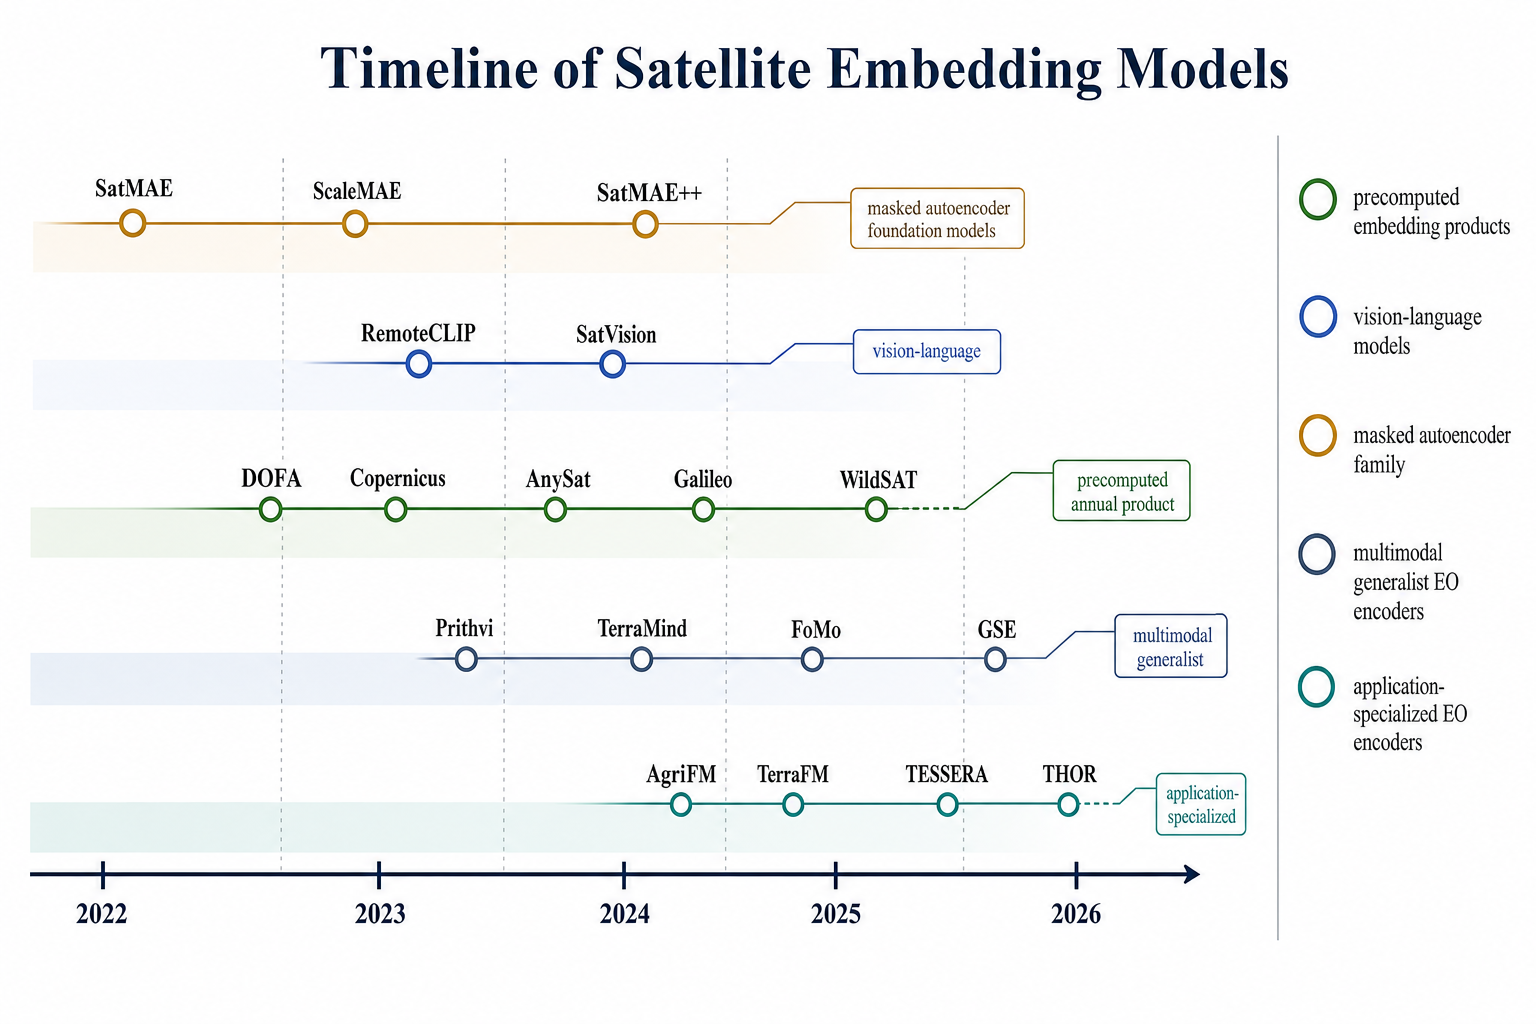
\includegraphics[width=\textwidth]{fig04_model_timeline_gptimage2_20260502.png}
  \caption{Model timeline view for the satellite embedding landscape. The figure emphasizes how precomputed products, masked autoencoder lineages, multimodal generalists, and application-specific encoders accumulate over time rather than appearing as a single homogeneous wave.}
  \label{fig:model-timeline}
\end{figure}

\subsection{Field evolution and major design axes}

For a remote sensing review, the overall story should appear before the detailed taxonomy. The field has evolved from early optical and masked-reconstruction pipelines toward broader multimodal, temporal, vision-language, and productized embedding systems. \figref{fig:model-timeline} provides this overall chronological view, which is easier for readers to absorb than a flat list of models.

We organize the literature along three orthogonal axes.

\paragraph{Model family.}
The first axis groups models by how the representation is learned and exposed: precomputed embedding products \citep{gse,tessera,copernicus}, vision-language systems \citep{remoteclip,wildsat}, masked autoencoder derivatives \citep{satmae,satmaepp,scalemae}, multimodal generalist encoders \citep{anysat,galileo,prithvi,terrafm,terramind,dofa}, and application-specialized Earth observation encoders \citep{agrifm,fomo,thor,satvision}.

\paragraph{Data and modality.}
The second axis captures the sensing substrate. Current models differ in optical-only versus optical-plus-SAR support, single-scene versus time-series modeling, fixed spectral assumptions versus wavelength-aware adaptation, and fine-resolution surface imagery versus coarse-resolution all-sky or atmosphere-linked sensing.

\paragraph{Deployment mode.}
The third axis separates systems that run a neural encoder at query time from systems that distribute the embedding directly as a product. This distinction is central for benchmarking because it changes runtime, storage, temporal flexibility, and failure modes. A precomputed product may offer extremely fast access but less temporal control, while an on-the-fly encoder may provide higher flexibility at the cost of data loading and GPU latency.

\begin{figure}[t]
  \centering
  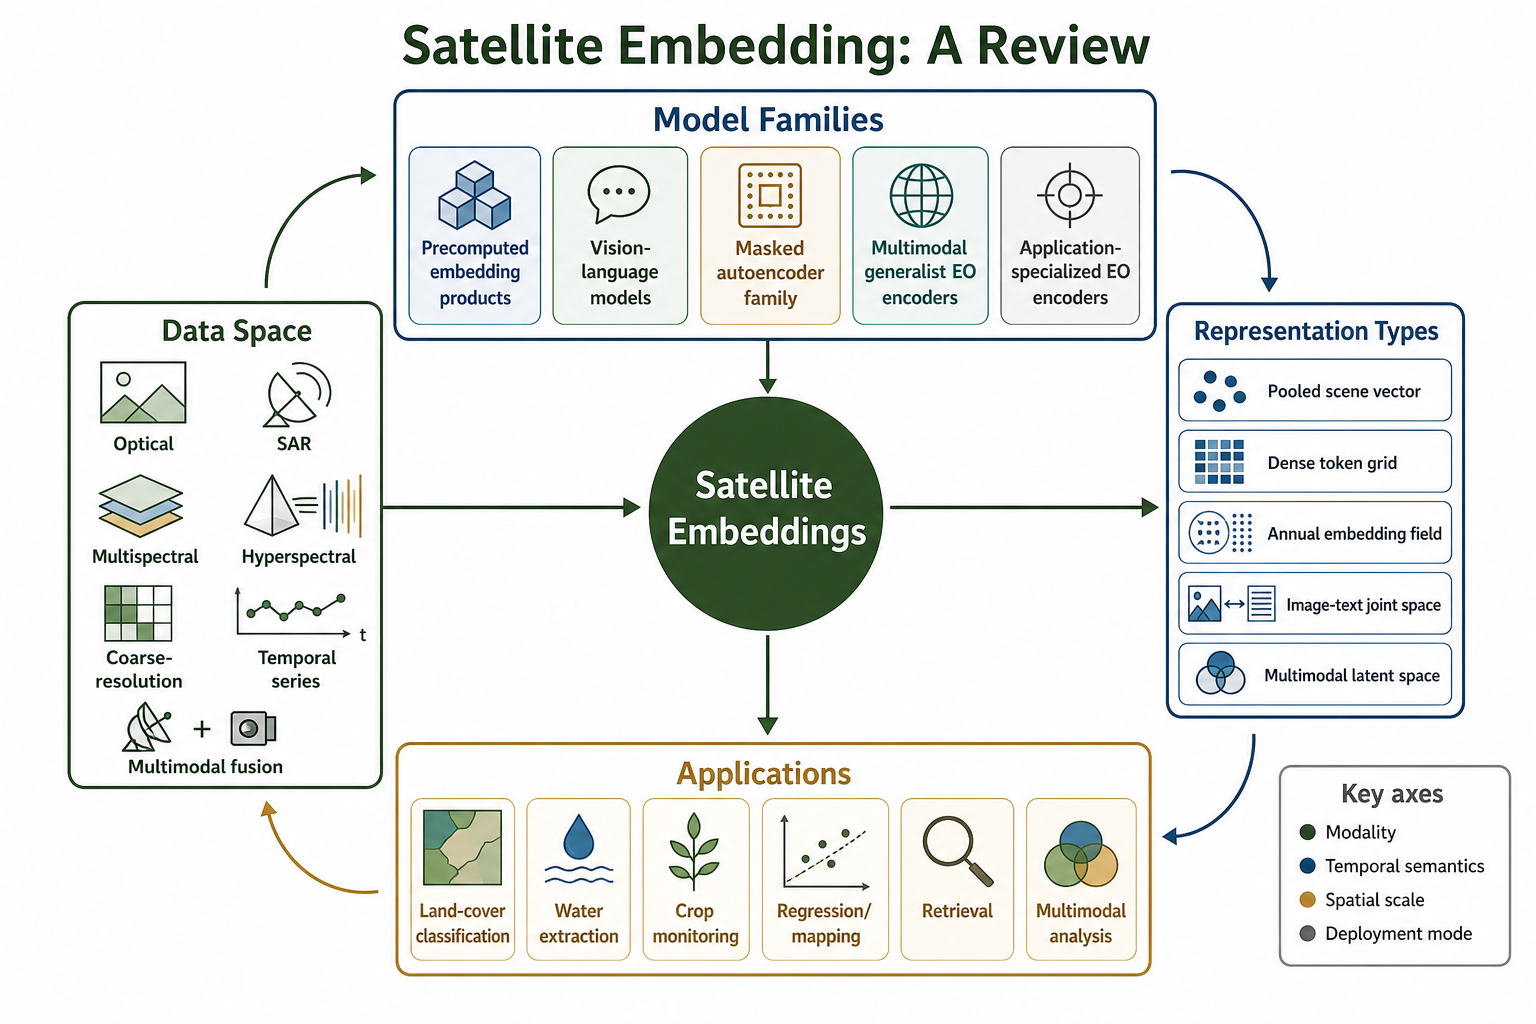
\includegraphics[width=\textwidth]{fig01_taxonomy_concept_map_gptimage2_20260502.png}
  \caption{Conceptual map of the satellite embedding landscape. The review is structured around four linked components: data space, model family, representation type, and downstream application. This framing is intentionally embedding-centered rather than checkpoint-centered.}
  \label{fig:taxonomy-concept-map}
\end{figure}

\subsection{Scope of this review}

An embedding-centered review should not simply relabel all remote sensing foundation models as satellite embeddings. Instead, the central question is whether the representation can serve as a general interface for downstream use. This criterion explains why annual products such as GSE and TESSERA belong in the same discussion as encoder checkpoints such as SatMAE++, AnySat, or TerraFM. All of them provide a transferable representation layer, but they differ sharply in spatial scale, temporal semantics, and deployment assumptions. \figref{fig:taxonomy-concept-map} summarizes this review logic in one diagram.

\section{Model Families of Satellite Embeddings}

The current \texttt{rs-embed} workspace exposes \modelcount{} canonical models, and the accompanying dossier records their publication metadata, supported sensors, output forms, and runtime summaries. For a review article, however, the reader should not face these as a flat inventory. A more natural structure is to first divide the field into a few broad model families, then summarize the common architecture and data logic of each family, and only after that return to a unified comparison table.

\subsection{Family I: Precomputed embedding products}

This family treats the embedding itself as a distributed geospatial product rather than as a checkpoint that must be run by the user. Examples include GSE, TESSERA, and Copernicus-style feature maps \citep{gse,tessera,copernicus}. Their main strengths are immediate access, large-area consistency, and low inference burden at use time. Their main limitations are temporal rigidity, storage requirements, and dependence on a fixed upstream production workflow.

\begin{figure}[t]
  \centering
  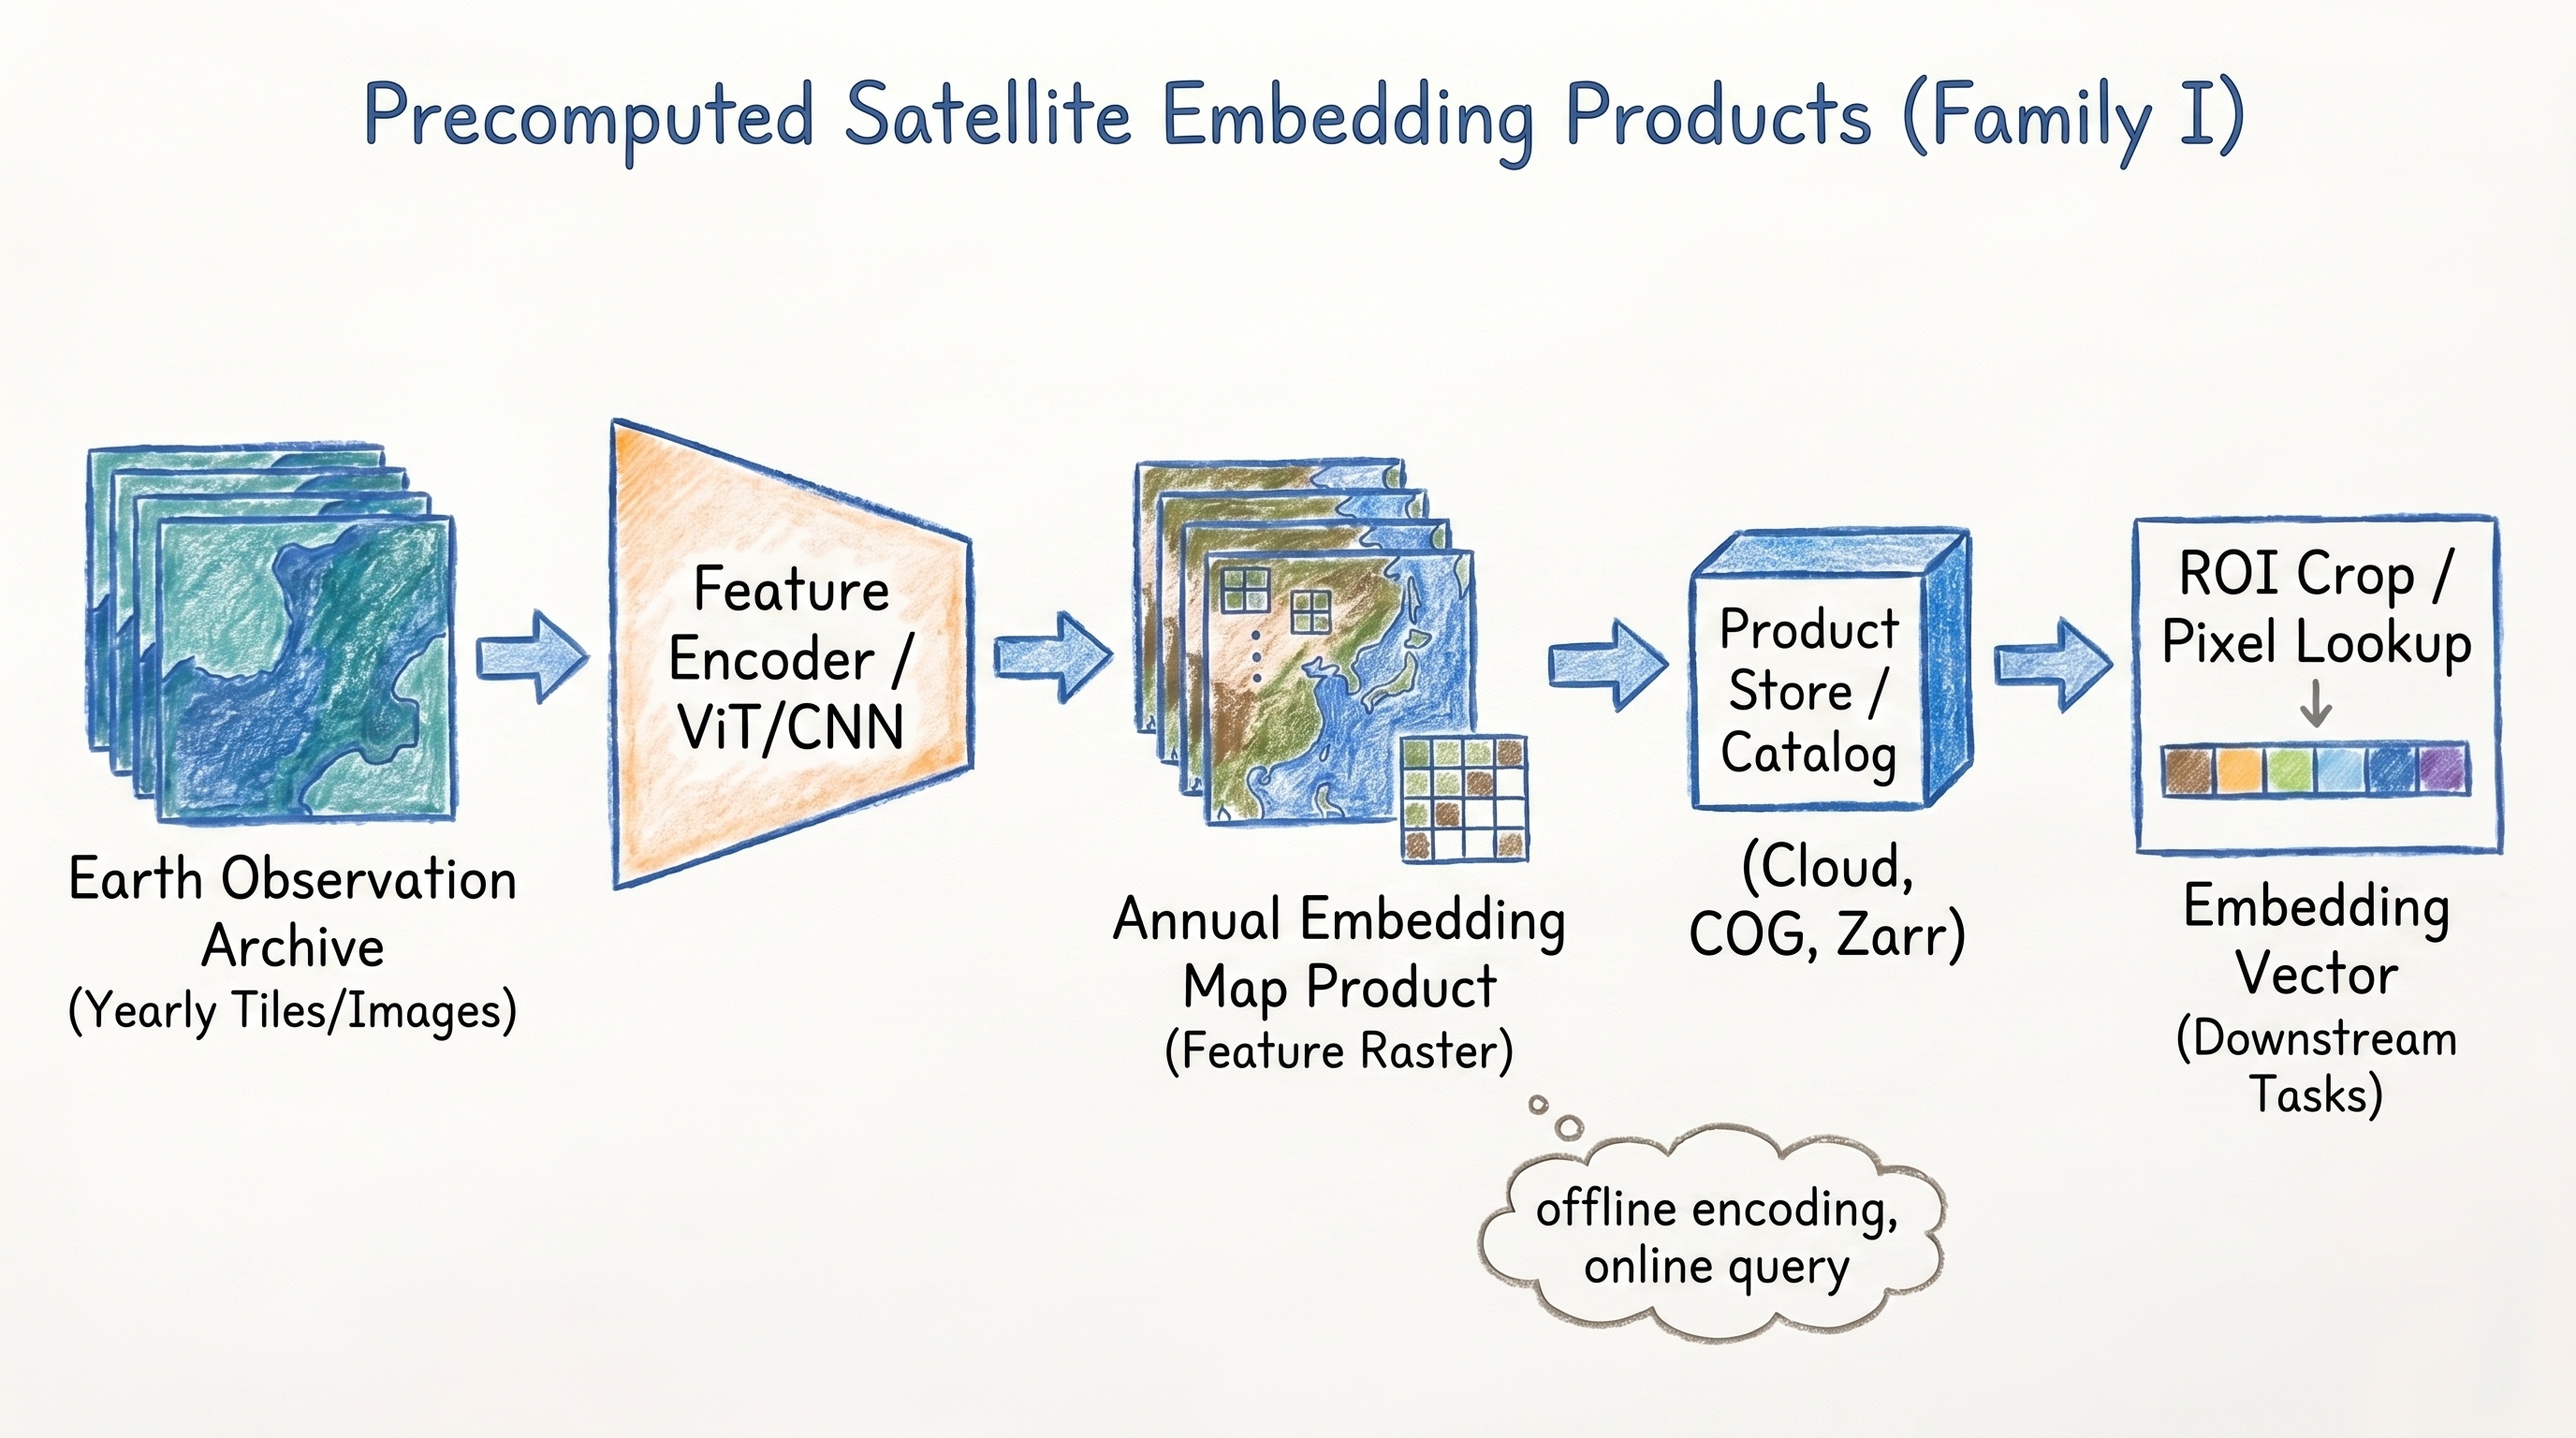
\includegraphics[width=\textwidth]{fig06_family_precomputed_products.png}
  \caption{Unified architecture sketch for precomputed embedding products. The dominant pattern is offline large-scale representation learning followed by annual or static embedding map generation, cataloging, and fast ROI-level feature access.}
  \label{fig:family-precomputed-products}
\end{figure}

\paragraph{Architecture summary.}
As summarized in \figref{fig:family-precomputed-products}, the central architectural move is to shift most computation from user-time to production-time. A large Earth observation archive is first condensed into a precomputed feature layer, often annualized or otherwise temporally summarized. Downstream users query that layer by ROI, tile, or pixel rather than rerunning the encoder. This architecture is especially attractive for wide-area monitoring and rapid transfer when access latency matters more than flexible temporal conditioning.

\paragraph{Pseudo-code template.}
\begin{pseudocode}
Input:
  Earth observation archive A
  temporal grouping rule T
  query ROI q

Offline stage:
  train encoder f_theta on large EO archive A
  for each period t in T:
      E_t <- f_theta(A_t)
      store embedding map E_t in product catalog

Online stage:
  crop or sample features z <- E_t[q]
  optionally pool or aggregate z
  train lightweight head g on sampled embeddings
  return prediction or retrieved features
\end{pseudocode}

\subsection{Family II: Masked autoencoder and pure vision encoders}

This group includes models such as SatMAE, SatMAE++, and ScaleMAE \citep{satmae,satmaepp,scalemae}. These methods are usually strongest when the goal is to learn transferable visual structure from optical or multispectral imagery through reconstruction-style pretraining. They are also among the clearest examples of the modern remote sensing foundation model trend, and many later systems can be interpreted as extending this lineage in scale, modality, or temporal handling.

\begin{figure}[t]
  \centering
  \includegraphics[width=\textwidth]{fig07_family_masked_autoencoder.png}
  \caption{Unified architecture sketch for masked autoencoder and pure vision satellite embedding models. Satellite tiles are partially masked, encoded by a transformer-style vision backbone, and supervised through reconstruction while the latent tokens are reused as transferable embeddings.}
  \label{fig:family-mae}
\end{figure}

\paragraph{Architecture summary.}
The shared logic in \figref{fig:family-mae} is to learn a compact latent representation from partial visual evidence. Randomly masked patches, channels, or scale-aware inputs are passed through a vision encoder, while a reconstruction module encourages the latent space to preserve transferable visual structure. These embeddings often work well for classification and segmentation because they retain strong spatial cues without requiring language supervision.

\paragraph{Pseudo-code template.}
\begin{pseudocode}
Input:
  satellite tile x
  masking policy M

visible, hidden <- apply_mask(x, M)
tokens <- patch_embed(visible)
latent <- encoder(tokens)
recon <- decoder(latent, hidden)
loss <- reconstruction_loss(recon, x)
update model parameters

at inference:
  z_pool, z_grid <- read encoder representations
  return transferable embedding features
\end{pseudocode}

\subsection{Family III: Vision-language and cross-modal embeddings}

\begin{figure}[t]
  \centering
  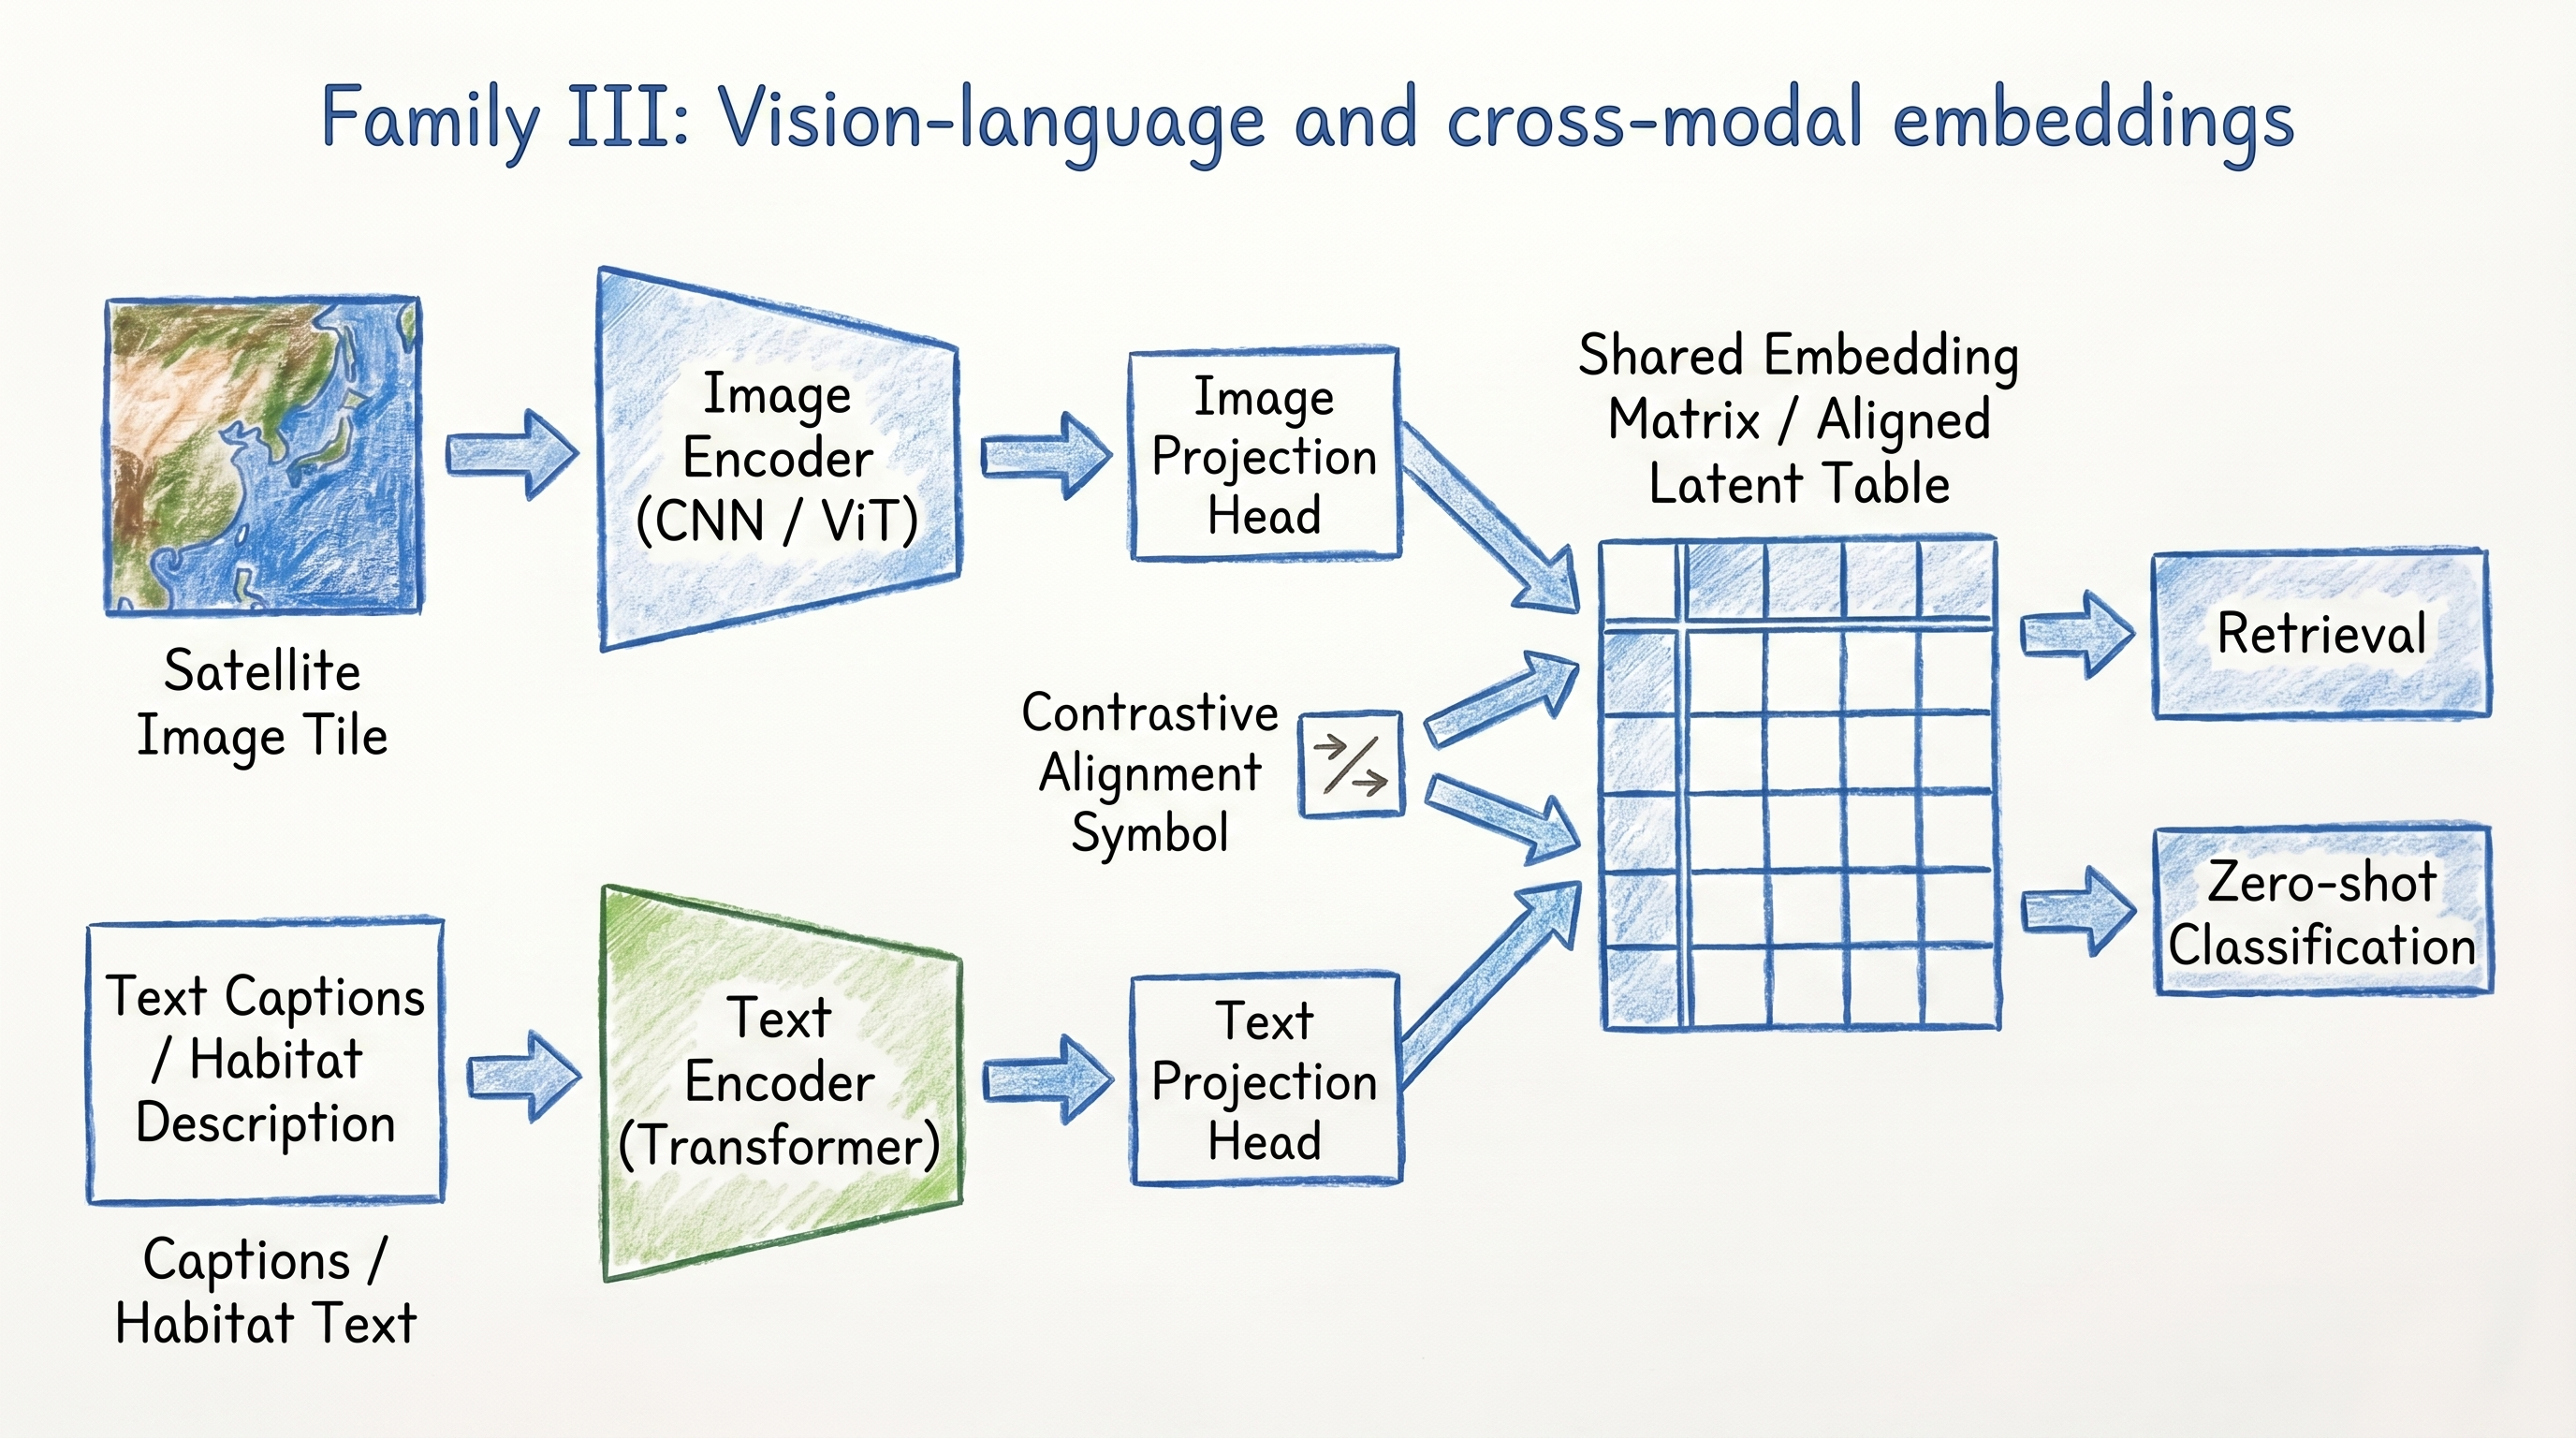
\includegraphics[width=\textwidth]{fig08_family_vision_language.png}
  \caption{Unified architecture sketch for vision-language and cross-modal satellite embeddings. The core pattern is image and text or ecological side-information encoding into a shared latent space trained by contrastive or alignment objectives.}
  \label{fig:family-vision-language}
\end{figure}

RemoteCLIP and WildSAT \citep{remoteclip,wildsat} illustrate the main idea of this family: satellite imagery is no longer embedded only against itself, but aligned with text, captions, habitat descriptions, or ecological side observations. \figref{fig:family-vision-language} shows this shared alignment pattern. This changes the representation from a purely visual latent space into a semantic one, which is why these models are especially important for retrieval, zero-shot transfer, and open-vocabulary interaction.

\paragraph{Architecture summary.}
Two encoders, one visual and one language or cross-modal, are trained to bring matched image-text or image-side-information pairs closer in a shared embedding space. The representation becomes useful not just for supervised transfer but also for semantic search and weakly supervised reasoning. In practice, this family adds a form of interpretability and open-vocabulary access that reconstruction-only models typically lack.

\paragraph{Pseudo-code template.}
\begin{pseudocode}
Input:
  satellite image x
  text or side-information y

z_img <- image_encoder(x)
z_txt <- text_encoder(y)
loss <- contrastive_alignment(z_img, z_txt)
update both encoders

at inference:
  use z_img for retrieval, zero-shot matching, or downstream probes
  optionally compare z_img against text prompt embeddings
\end{pseudocode}

\subsection{Family IV: Multimodal generalist EO encoders}

AnySat, Galileo, Prithvi, TerraFM, TerraMind, and DOFA represent a broader push toward modality-flexible or sensor-flexible Earth observation representation learning \citep{anysat,galileo,prithvi,terrafm,terramind,dofa}. These models are important because they move the field closer to a genuinely general EO representation space. Their distinguishing features include explicit handling of temporal stacks, wavelength metadata, modality routing, and cross-sensor alignment.

\begin{figure}[t]
  \centering
  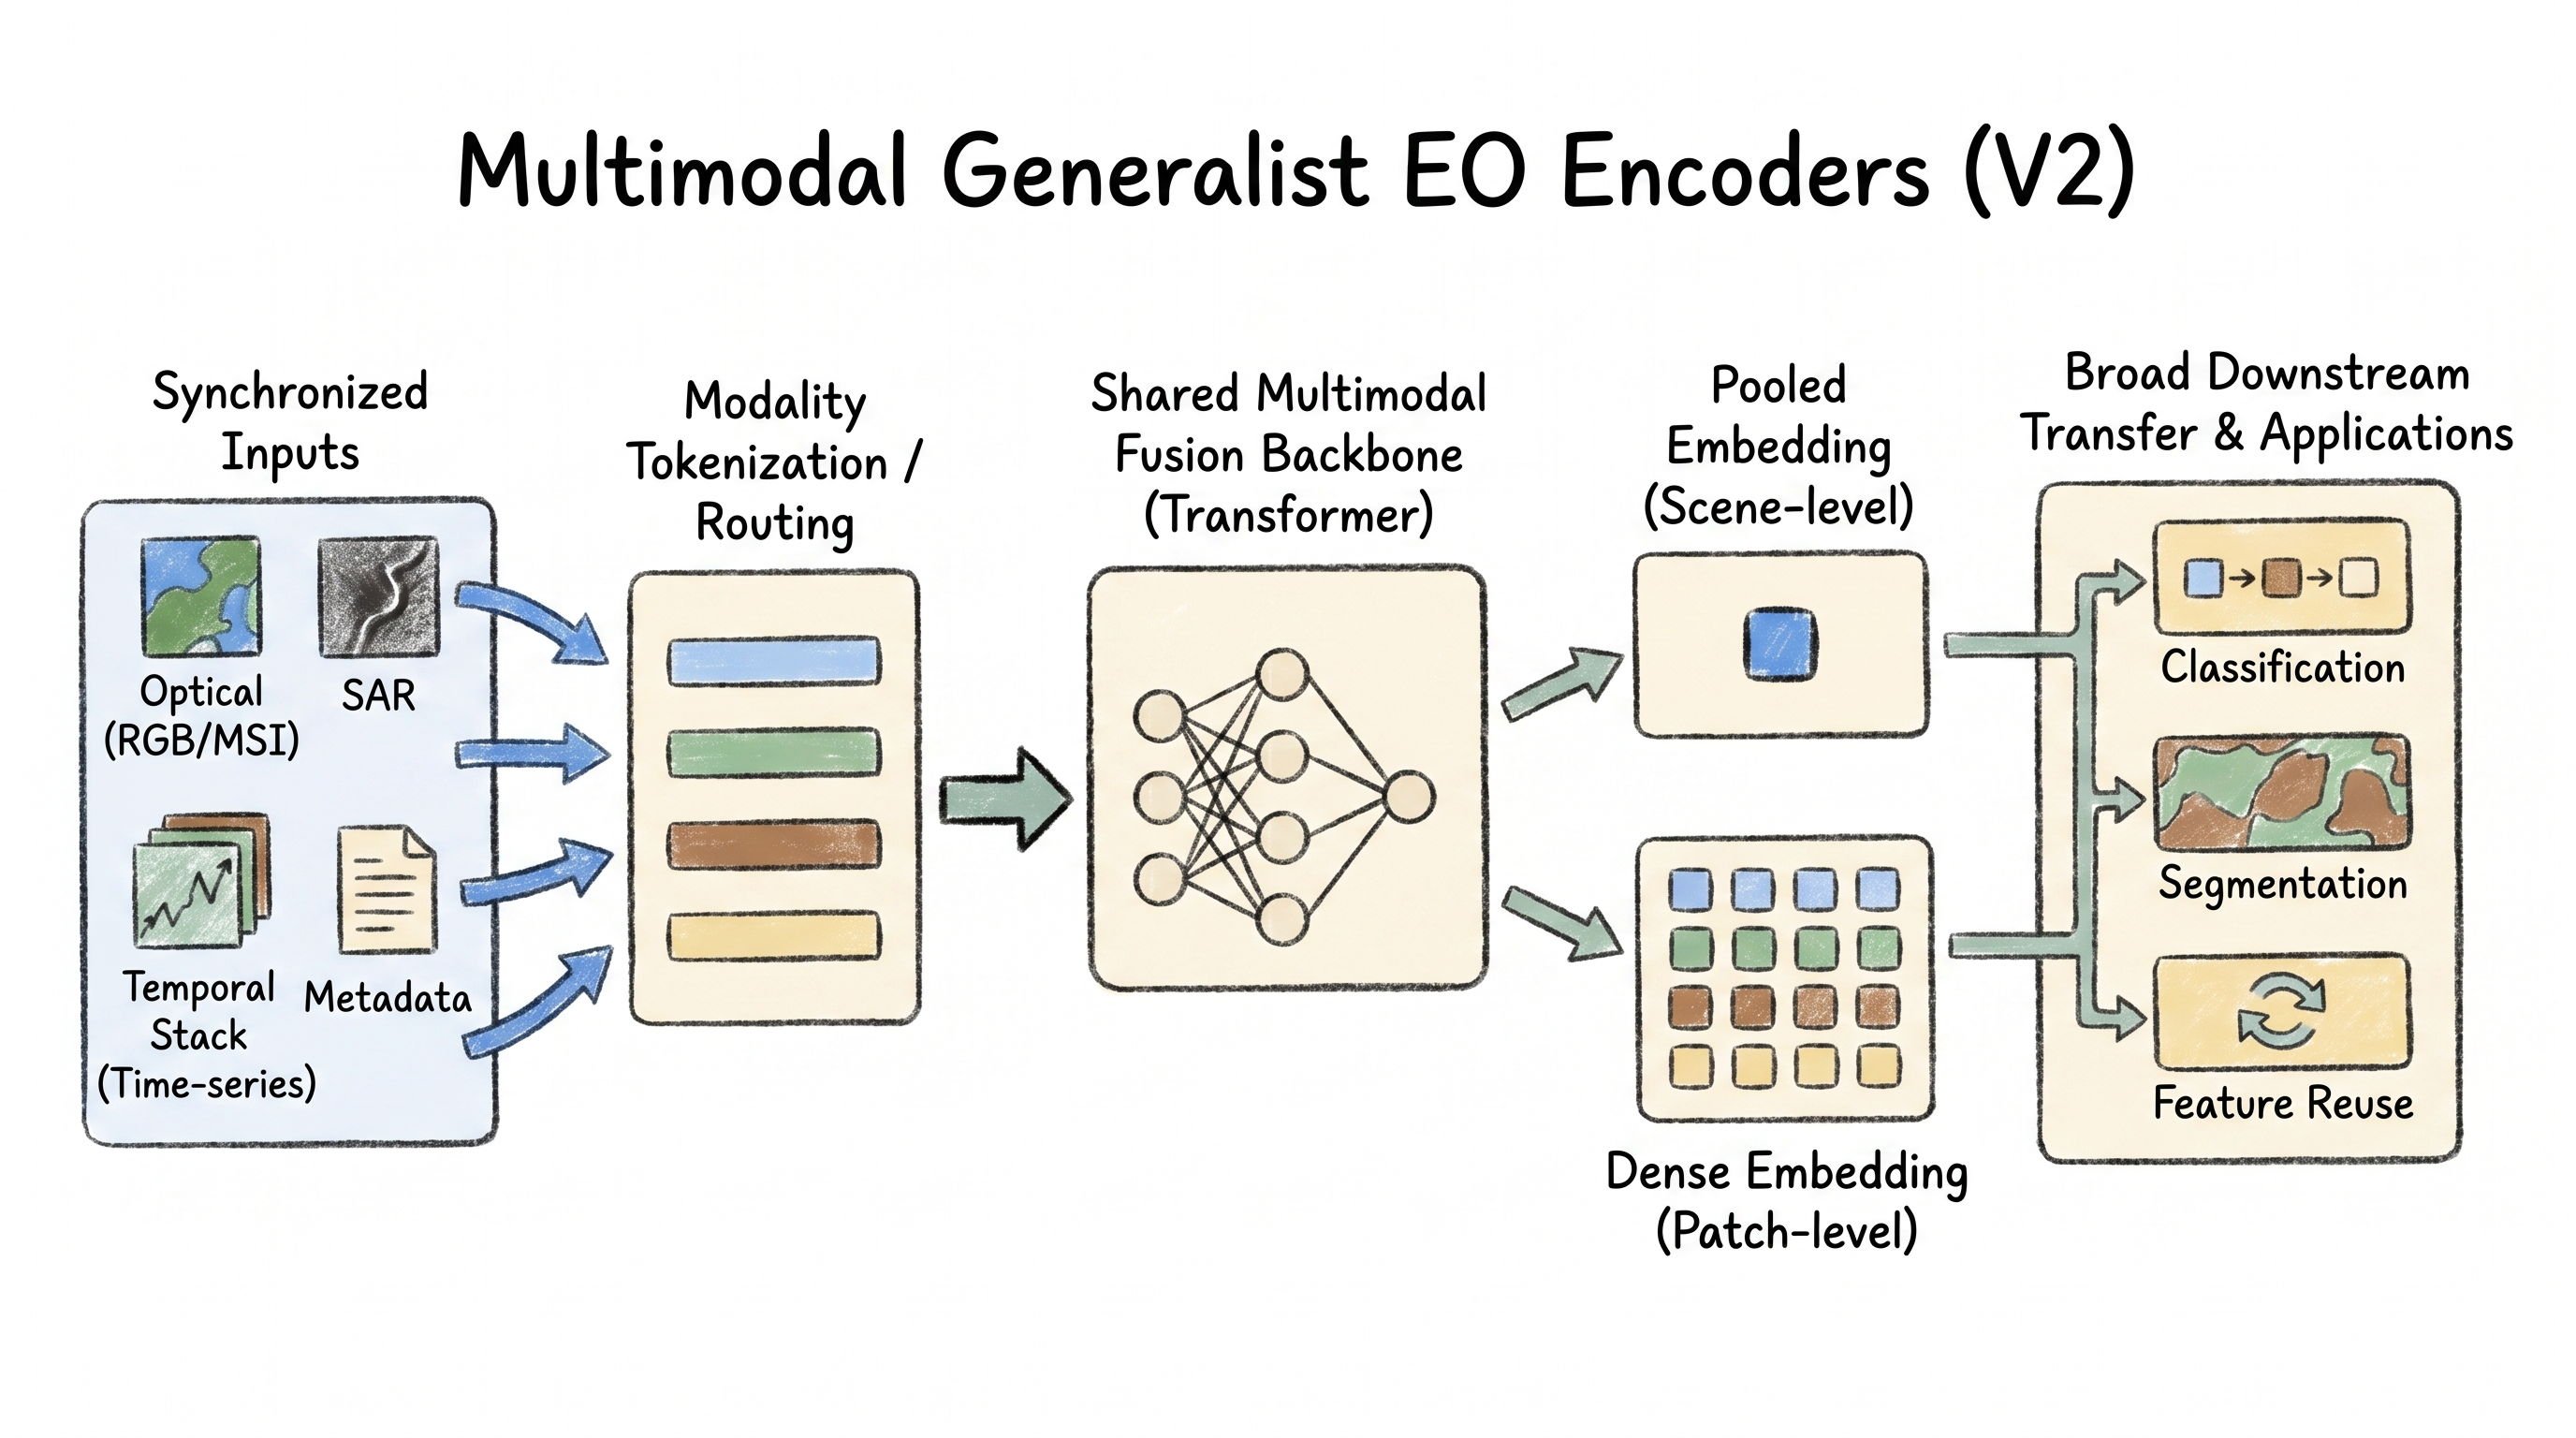
\includegraphics[width=\textwidth]{fig09_family_multimodal_generalist.png}
  \caption{Unified architecture sketch for multimodal generalist EO encoders. Multiple sensor streams are tokenized, routed or aligned, fused by a shared backbone, and exported as pooled or dense representations for broad downstream transfer.}
  \label{fig:family-generalist}
\end{figure}

\paragraph{Architecture summary.}
As \figref{fig:family-generalist} summarizes, the defining goal of this family is not simply to process more inputs, but to learn a common representation space across sensors, scales, time, and metadata. Architecturally, that often means modality-specific tokenization combined with a shared transformer or fusion backbone. These models are closest to a true Earth observation foundation layer because they seek one latent space that remains useful under heterogeneous sensing conditions.

\paragraph{Pseudo-code template.}
\begin{pseudocode}
Input:
  modalities {x_1, x_2, ..., x_m}
  temporal or metadata context c

for each modality x_i:
    t_i <- modality_tokenizer_i(x_i, c)

t_shared <- temporal_align_and_route({t_i}, c)
h <- multimodal_backbone(t_shared)
z_pool, z_grid <- readout(h)
optimize self-supervised or multimodal objective

return shared embeddings for cross-sensor downstream transfer
\end{pseudocode}

\subsection{Family V: Domain-specialized embedding models}

Not all useful satellite embeddings aim at maximal generality. AgriFM, FoMo, THOR, and SatVision show that domain-oriented models can remain highly valuable when their sensor assumptions and application context are well matched \citep{agrifm,fomo,thor,satvision}. In a remote sensing review, these models should appear as a major family rather than as outliers, because they often reflect the real structure of EO practice: agriculture, forestry, biodiversity, atmosphere, climate, and societal monitoring all impose different representation demands.

\begin{figure}[t]
  \centering
  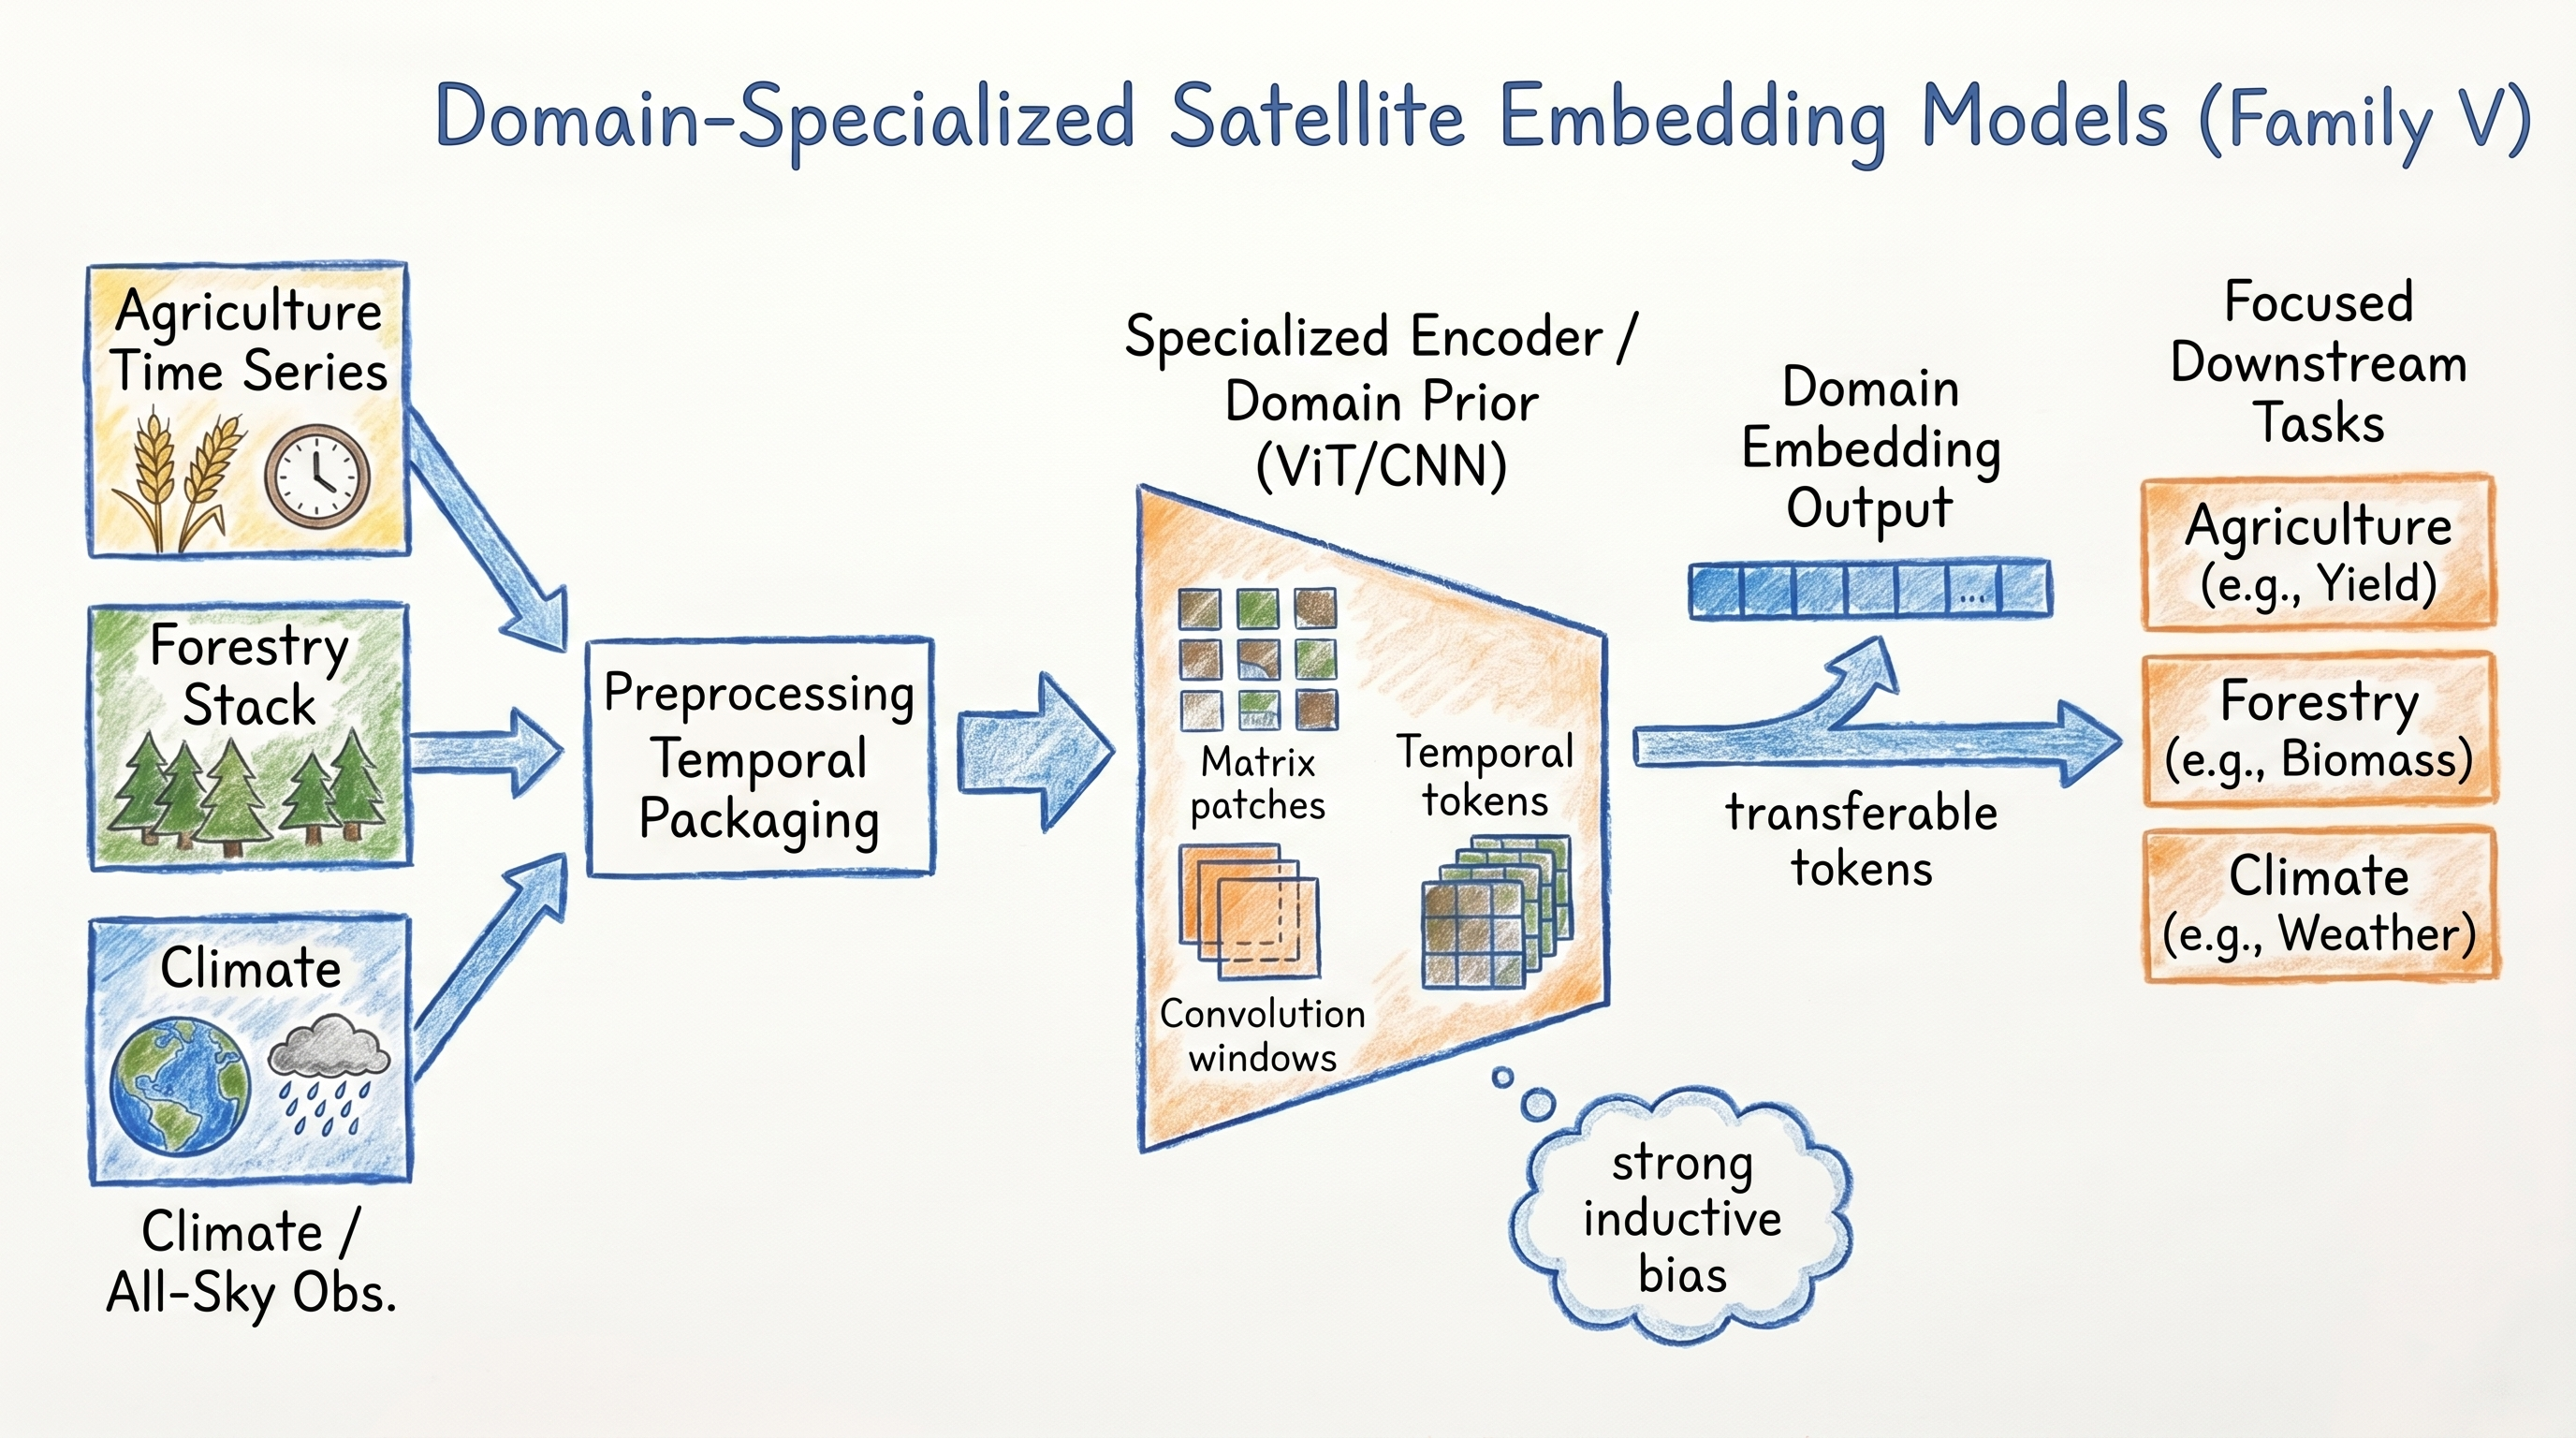
\includegraphics[width=\textwidth]{fig10_family_specialized.png}
  \caption{Unified architecture sketch for domain-specialized satellite embedding models. Domain-specific sensing pipelines and inductive biases are used to produce embeddings that are narrower in scope but often better matched to particular application regimes.}
  \label{fig:family-specialized}
\end{figure}

\paragraph{Architecture summary.}
As sketched in \figref{fig:family-specialized}, this family accepts a narrower operating domain in exchange for stronger inductive bias. Agricultural time series, forest monitoring stacks, climate-oriented inputs, or coarse all-sky observations are processed with task-aware temporal packaging, scale handling, or specialized supervision. These models remind us that the best EO embedding is not always the most general one; in many real applications, domain fit matters more than universality.

\paragraph{Pseudo-code template.}
\begin{pseudocode}
Input:
  domain-specific sensor stream x
  domain labels or weak supervision y
  domain prior pi

x_tilde <- domain_preprocess(x, pi)
h <- specialized_encoder(x_tilde, pi)
z <- domain_embedding_head(h)
loss <- domain_objective(z, y, pi)
update model parameters

at deployment:
  reuse z for domain-focused mapping, monitoring, or regression
\end{pseudocode}

\subsection{Cross-family comparison}

After the family-level discussion, the review can return to a unified comparison table. This ordering is closer to the way remote sensing surveys are usually read: first understand the main branches of the field, then inspect the full inventory.

Table~\ref{tab:model-catalog} turns the structured dossier into a paper-ready catalog. Unlike a compact leaderboard, it keeps the deployment type, sensing assumptions, temporal semantics, and pretraining regime visible, because these details strongly determine whether a model is suitable for retrieval, dense prediction, or operational mapping.

\begin{landscape}
\scriptsize
\setlength{\LTleft}{0pt}
\setlength{\LTright}{0pt}
\setlength{\tabcolsep}{3pt}
\renewcommand{\arraystretch}{1.15}
\begin{longtable}{p{1.45cm}p{0.75cm}p{1.2cm}p{0.95cm}p{2.25cm}p{2.05cm}p{2.75cm}p{2.35cm}p{2.25cm}p{1.55cm}p{3.0cm}}
\caption{Comprehensive model summary for the \modelcount{} canonical satellite embedding models currently exposed in \texttt{rs-embed}. The table emphasizes deployment-relevant details rather than only benchmark scores.}\label{tab:model-catalog}\\
\toprule
Model & Year & Venue & Type & Family & Backbone & Sensors / data & Resolution & Temporal semantics & Emb. / output & Pretraining signal \\
\midrule
\endfirsthead
\caption[]{Comprehensive model summary for the canonical \texttt{rs-embed} model set (continued).}\\
\toprule
Model & Year & Venue & Type & Family & Backbone & Sensors / data & Resolution & Temporal semantics & Emb. / output & Pretraining signal \\
\midrule
\endhead
\bottomrule
\endfoot
tessera & 2026 & CVPR & precomputed & Precomputed temporal embedding field & field model over surface spectra embeddings & surface spectra product & 10 m precomputed embedding tiles & annual lookup over product years & 128; pooled, grid & embedding field regression / product training \\
gse & 2025 & arXiv & precomputed & Precomputed annual embedding product & embedding field model & Google Satellite Embedding annual product & 10 m annual embedding product & strict yearly product & 64; pooled, grid & global embedding field learning from sparse labels \\
copernicus & 2025 & ICCV & precomputed & Precomputed foundation map & Copernicus foundation model product & Copernicus product stack & 0.25\textdegree{} precomputed grid & static in current adapter (2021 only) & 768; pooled, grid & foundation model pretraining followed by product distillation \\
remoteclip & 2024 & IEEE TGRS & on-the-fly & Vision-language satellite embedding & CLIP / ViT-B-32 & Sentinel-2 RGB, remote sensing captions, UAV imagery in pretraining & 10 m; Sentinel-2 RGB & single composited observation window at inference & 768; pooled, grid & contrastive image-text alignment (InfoNCE) \\
satmae & 2022 & NeurIPS & on-the-fly & Masked autoencoder for temporal or multispectral EO & ViT-MAE & Sentinel-2 RGB or multispectral/time-series variants in original paper & 10 m; Sentinel-2 RGB & explicit temporal embeddings in the original paper; rs-embed adapter currently uses RGB composite path & 1024; pooled, grid & masked autoencoding with temporal/spectral positional encoding \\
satmaepp & 2024 & CVPR & on-the-fly & Improved masked autoencoder for EO & ViT-L / SatMAE++ & Sentinel-2 RGB in adapter, multispectral Sentinel-2 in paper & 10 m; Sentinel-2 RGB & single composited observation window in adapter & 1024; pooled, grid & revised MAE pretraining for multispectral satellite imagery \\
satmaepp\_s2\_10b & 2024 & CVPR & on-the-fly & Grouped-channel multispectral masked autoencoder & ViT-L / grouped-channel SatMAE++ & Sentinel-2 SR 10-band & 10 m; Sentinel-2 SR 10-band input & single composited observation window in adapter & 1024; pooled, grid & grouped-channel masked autoencoding \\
scalemae & 2023 & ICCV & on-the-fly & Scale-aware masked autoencoder & ViT-L / MAE & Sentinel-2 RGB in adapter, multiscale EO imagery in paper & 10 m; Sentinel-2 RGB, plus explicit semantic scale input & single composited observation window & 1024; pooled, grid & masked autoencoding with explicit resolution conditioning \\
anysat & 2025 & CVPR & on-the-fly & Generalist multi-resolution multimodal EO encoder & versatile JEPA-style EO encoder & Sentinel-2, Sentinel-1, aerial/VHR and other modalities in original paper & 10 m Sentinel-2 time-series input; default per-frame resize 24 px & multi-frame optical sequence with date tokens & 768; pooled, grid & self-supervised representation learning across many configurations \\
galileo & 2025 & ICML & on-the-fly & Global-local multimodal time-series encoder & transformer with global/local branches & Sentinel-2 time series, multiple remote sensing modalities in original work & 10 m Sentinel-2 time-series input; default frame size 64 px, patch size 8 & explicit month tokens and frame masks & 128; pooled, grid & self-supervised multimodal representation learning \\
wildsat & 2025 & ICCV & on-the-fly & Remote sensing representation learning from weak labels & ViT-B-16 & Sentinel-2 RGB, wildlife observations as supervision & 10 m; Sentinel-2 RGB & single composited optical patch & 256; pooled, grid & supervised / weakly supervised representation learning from wildlife observations \\
prithvi & 2023 & arXiv & on-the-fly & Generalist geospatial foundation model & ViT / masked autoencoder lineage & HLS / Sentinel-Landsat style 6-band optical imagery & 30 m in current adapter; Sentinel-2 6-band input & explicit temporal coordinates in adapter and paper family & 768; pooled, grid & self-supervised geospatial pretraining \\
terrafm & 2026 & ICLR & on-the-fly & Unified multisensor foundation model & multisensor transformer & Sentinel-2, Sentinel-1 & 10 m for both S2 and S1 paths; image resized to 224 px & single observation window in current adapter; paper focuses on multisensor unification & 768; pooled, grid & scalable unified multisensor pretraining \\
terramind & 2025 & ICCV & on-the-fly & Generative multimodal EO foundation model & large-scale generative multimodal transformer & Sentinel-2 in adapter, wider multimodal EO stack in paper & 10 m; Sentinel-2 SR 12-band input; image resized to 224 px & single composited optical path in adapter & 384; pooled, grid & large-scale generative multimodal learning \\
dofa & 2024 & arXiv & on-the-fly & Wavelength-aware multimodal foundation model & transformer with neural plasticity / dynamic wavelength handling & multispectral and hyperspectral style inputs, Sentinel-2 in adapter & 10 m for S2 path; fixed resize to 224 px & single observation window in adapter & 768; pooled, grid & self-supervised multimodal EO foundation modeling \\
fomo & 2025 & AAAI & on-the-fly & Forest-oriented multimodal and multiscale foundation model & multimodal transformer / representation learner & Sentinel-2 SR in adapter, multiple scales and tasks in original work & 10 m; Sentinel-2 SR 12-band input; default image size 64 px & single optical composite in adapter & 768; pooled, grid & multi-task forest monitoring pretraining \\
thor & 2026 & arXiv & on-the-fly & Versatile EO foundation model for climate and society & versatile transformer & Sentinel-2 SR 10-band & 10 m; Sentinel-2 SR 10-band input; default image size 288 px & single optical composite in adapter & 768; pooled, grid & foundation pretraining for climate and society applications \\
agrifm & 2026 & Remote Sensing of Environment & on-the-fly & Agriculture-specific multi-source temporal foundation model & Video Swin Transformer & Sentinel-2 in adapter, Sentinel-2, Landsat-8/9, MODIS in original paper & 10 m Sentinel-2 time-series input; default image size 224 px with fixed T-frame packaging & fixed-length multi-frame temporal stack & 1024; pooled, grid & supervised land-cover fraction pretraining with EMA teacher \\
satvision & 2024 & arXiv & on-the-fly & Coarse-resolution all-sky foundation model & SwinV2-style encoder & MODIS 14-band TOA & 1000 m; 14-channel TOA input & single coarse-resolution observation window in adapter & 4096; pooled, grid & foundation pretraining on all-sky MODIS TOA data \\
\end{longtable}
\normalsize
\end{landscape}


Three contrasts recur across families. First, precomputed layers prioritize access and coverage, while on-the-fly encoders prioritize flexibility. Second, multimodal and time-aware systems attempt to absorb sensor heterogeneity at training time, whereas narrower families often compensate with stronger specialization and simpler deployment. Third, vision-language models add open-vocabulary semantics that are mostly absent from pure masked reconstruction pipelines. These contrasts matter more for a review paper than a single benchmark leaderboard, because they explain why different families remain competitive under different downstream conditions.

\begin{figure}[t]
  \centering
  \includegraphics[width=\textwidth]{fig05_resolution_modality_matrix.png}
  \caption{Resolution-modality matrix for current satellite embedding models. The same model family can occupy very different parts of the sensing space, from coarse-resolution all-sky imagery to high-resolution optical-SAR or multimodal temporal embeddings.}
  \label{fig:resolution-modality-matrix}
\end{figure}

\figref{fig:resolution-modality-matrix} closes this section by summarizing the sensing space covered by current models. In a remote sensing context, this figure is often more informative than a single ranking table because it makes sensor assumptions and scale mismatch immediately visible.

\section{Data Resources, Application Space, and Evaluation Logic}

Recent remote sensing review articles in RSE, TGRS, and ISPRS tend to avoid treating methods, datasets, and applications as isolated lists. Instead, they first describe the sensing and data regime, then organize methodological families around the downstream questions that remote sensing users actually ask, and finally return to limitations, scale effects, and evaluation practice \citep{ma2019dl_meta_isprs,yuan2020env_dl_rse,weiss2020agri_meta_rse,paoletti2019hsi_review,li2020object_detection_isprs,survey1,xiao2025foundation_survey}. This organization is especially appropriate for satellite embeddings because an embedding is not a complete solution by itself. It is an intermediate representation whose usefulness depends on the sensor stream from which it was learned, the spatial and temporal scale at which it is exposed, and the type of downstream evidence that a user wants to recover. A pooled vector can be excellent for tile classification but insufficient for shoreline delineation; a dense feature grid can support segmentation but may be expensive or unavailable for some products; an annual precomputed layer can be ideal for wide-area screening but poorly matched to event-specific monitoring. The application section therefore has to do more than enumerate tasks. It must explain how the embedding form constrains the mapping problem.

The first organizing dimension is the data regime. Most current satellite embeddings are produced from one of four recurring sources: medium-resolution optical archives such as Sentinel-2 and Landsat, optical-SAR combinations centered on Sentinel-1 and Sentinel-2, broader multimodal stacks that add elevation, weather, labels, text, or metadata, and precomputed embedding products that have already collapsed a large archive into a queryable feature layer. These regimes create different forms of transfer. Optical-only models usually retain strong spectral and spatial cues for land-cover mapping, but they may fail under cloud, season, or sensor changes if temporal handling is weak. Optical-SAR and multimodal models try to absorb those changes during representation learning, but their practical value depends on whether all required inputs are available in the target region and period. Precomputed products shift the problem again: they reduce inference cost and make wide-area sampling simple, yet they also fix the upstream temporal summary, native scale, and production assumptions. This is why the same model family can behave very differently when evaluated at 10\,m, 30\,m, 500\,m, 1\,km, or 0.25$^\circ$ resolution. In an embedding-centered review, native scale is not a footnote; it is part of the representation.

The second organizing dimension is the downstream target. Classification and mapping remain the most common entry point because they are compatible with almost every embedding family. A single pooled vector per tile is often enough to support land-cover labels, crop categories, forest condition classes, urban typologies, or simple ecological strata. This makes classification a useful baseline, but it is also an incomplete test: a model can separate dominant classes while losing continuous mixture information or local boundary structure. Regression tasks address that gap by asking whether the embedding preserves smoothly varying quantities such as built-up fraction, vegetation fraction, biomass proxies, canopy height, crop-yield indicators, or environmental indices. Dense prediction tasks push further by asking whether the representation still contains spatially localized information after tokenization, pooling, product resampling, or temporal summarization. Water extraction, land-cover segmentation, flood mapping, and mask reconstruction are therefore not merely additional applications; they probe whether the embedding is a spatial representation rather than only a semantic descriptor. Finally, vision-language and cross-modal embeddings introduce retrieval and open-vocabulary search as a distinct mode of use. These tasks are promising, but they should be interpreted separately from supervised mapping because they measure semantic alignment and promptability rather than only geographic fidelity.

The third organizing dimension is operational fit. Remote sensing users rarely choose an embedding only because it has the highest number in a table. They also need to know whether the representation can be generated for the desired sensor, season, and region; whether it exposes pooled or dense outputs; whether it can be sampled as a product or requires GPU inference; whether runtime and memory scale with area; and whether the temporal meaning of the output is annual, seasonal, monthly, or scene-specific. Recent foundation-model surveys have emphasized the same concern from a broader model perspective, but embedding selection makes it even sharper: two systems can both be called foundation models while exposing very different reusable objects \citep{survey1,survey3,survey4,xiao2025foundation_survey}. The review therefore treats applications as representation tests. Classification tests semantic separability, regression tests continuous structure, binary extraction tests operational thresholdability, segmentation tests local spatial separability, and retrieval tests cross-modal alignment. This evaluation logic leads directly to the compact benchmark in the next section.

\section{A Compact Wuhan Benchmark for Satellite Embeddings}

The empirical component of this review is intentionally modest in geographic scope but strict in comparison logic. Rather than assembling unrelated benchmark numbers from model papers, we evaluate all \modelcount{} public models on one high-resolution Wuhan ROI covering the East Lake--Tangxun Lake corridor. The region is useful for a first controlled comparison because it contains a compact mixture of open water, dense urban fabric, vegetation, cropland, and mixed transition zones. That mixture is large enough to expose scale and representation differences, but small enough to make repeated extraction, cache checking, and visual inspection feasible. This follows the spirit of benchmark-oriented remote sensing reviews, where a local protocol is not presented as a substitute for global validation, but as a controlled lens for understanding how methods behave under shared data, labels, and evaluation rules \citep{li2020object_detection_isprs,cheng2016object_detection_isprs,reobench}.

All benchmark tasks use the same 500\,m tile grid, the same train/validation/test split, and lightweight heads fitted on frozen embeddings. The protocol deliberately avoids end-to-end fine-tuning because the goal is to compare the information already present in each reusable representation. On-the-fly encoders are run or cached over the same Wuhan window, while precomputed products are sampled at the nearest compatible temporal layer and resampled only as needed for the shared tile grid. This design makes the comparison fairer than reading model-paper leaderboards, but it also keeps the interpretation honest: the results describe local transfer under one urban-lake landscape, not universal model superiority. The benchmark is therefore best read as a diagnostic complement to the literature review. It asks which embeddings preserve class separability, continuous land-cover mixture, water/non-water thresholdability, and dense class structure when the geography, labels, and probe complexity are held fixed.

\begin{figure}[t]
  \centering
  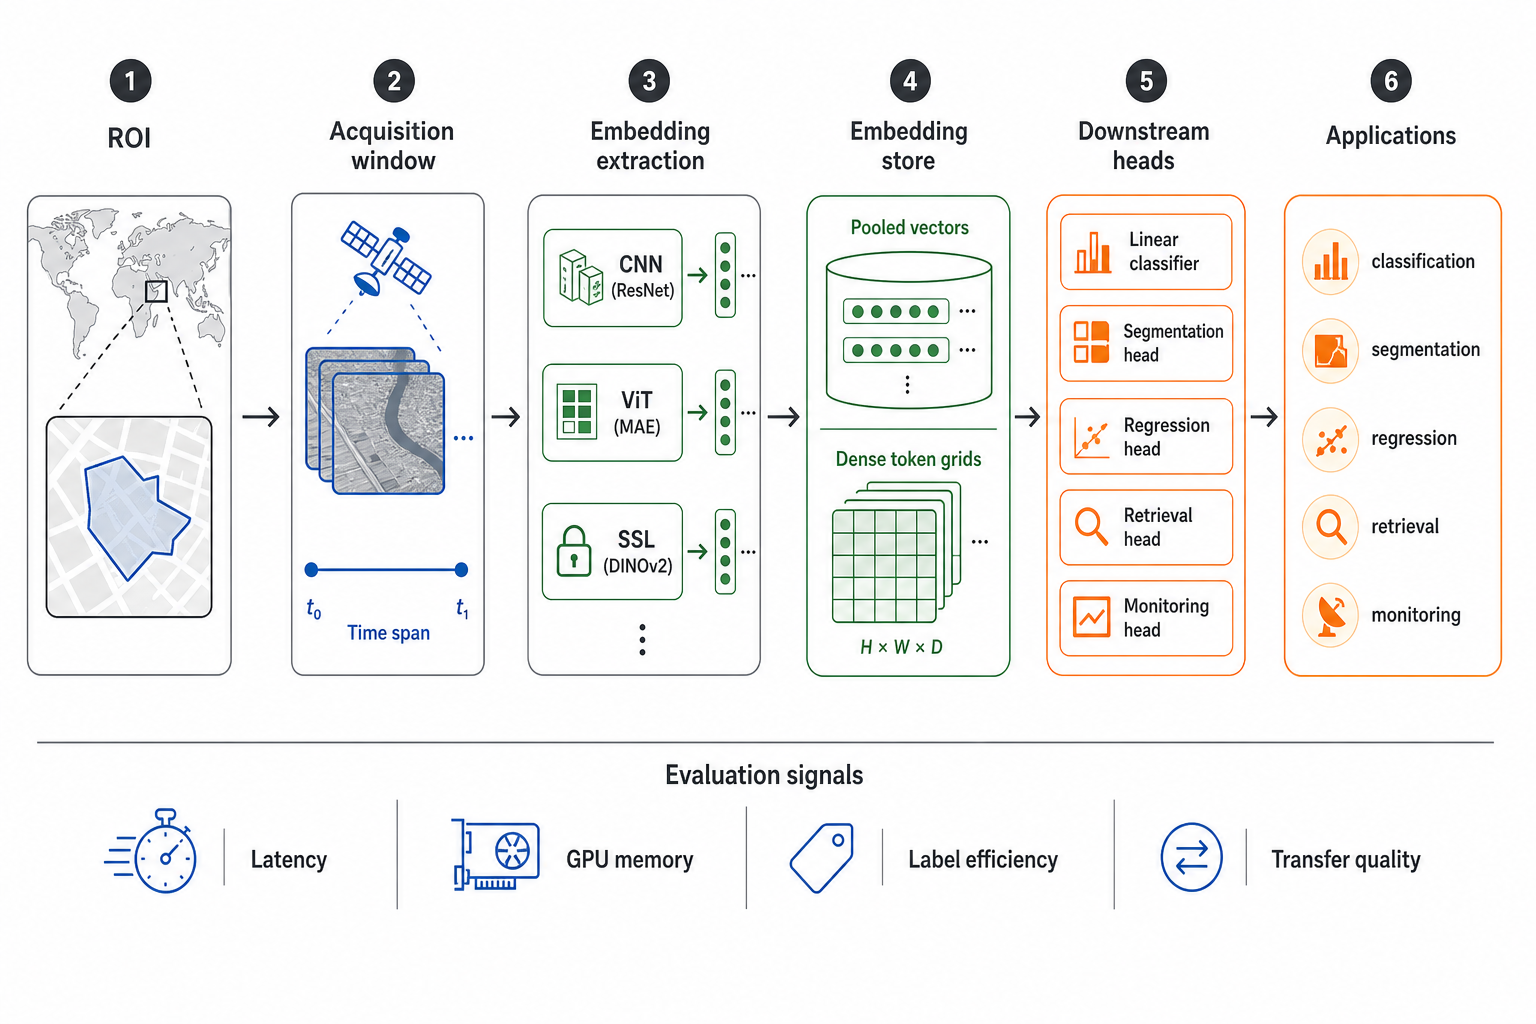
\includegraphics[width=\textwidth]{fig02_application_pipeline_gptimage2_20260502.png}
  \caption{Application-oriented benchmark pipeline. A shared region of interest is converted into a unified embedding extraction workflow, lightweight probe heads, and downstream evaluation targets spanning classification, segmentation, regression, and retrieval.}
  \label{fig:application-pipeline}
\end{figure}

the initial 15-tile pilot: it keeps the same region and label semantics, but
tests whether the observed model differences remain visible across a larger,
\figref{fig:application-pipeline} summarizes the benchmark pipeline. The executed version uses the current two-by-two Wuhan window, which expands the original visual sanity case to four adjacent Sentinel-2 blocks and 567 valid 500\,m tiles. Labels are derived from ESA WorldCover 2021 and JRC Global Surface Water, then converted into four related evaluation views: dominant land-cover classification, built-up/vegetation/cropland/water fraction regression, binary water extraction, and dense multi-class threshold segmentation. These tasks are deliberately related rather than independent. The same tile that is easy to classify as water may still be difficult near a mixed shoreline; the same embedding that ranks vegetation fraction well may still blur cropland boundaries; and the same product that looks coherent in a map may fail when its native grid is too coarse for 500\,m probing. Using related tasks over one ROI therefore makes the benchmark more diagnostic than a collection of disconnected scores.

\figref{fig:wuhan-2x-embedding-overview} provides the visual acceptance
case for this expanded benchmark before any downstream probe is fitted. The
upper-left reference panel shows the original 2x Wuhan window, while the
remaining panels show the corresponding model-specific embedding maps for the
\modelcount{} public models. The comparison is intentionally qualitative: it
checks whether the exported embeddings preserve a recognizable spatial
organization over the same geographic footprint. Several models recover the
lake corridor and surrounding urban-vegetation contrast as coherent regions,
whereas coarser or less spatially matched representations appear flatter,
blockier, or less locally structured. This figure therefore establishes that
the downstream classification and regression tasks are being run on a common
region where the models already expose visibly different spatial behavior.

\begin{figure}[t]
  \centering
  \includegraphics[width=\textwidth]{fig10_wuhan_2x_embedding_overview.png}
  \caption{Original imagery and public-model embedding maps for the two-by-two
  Wuhan benchmark window. The reference image anchors the shared geographic
  footprint, and the remaining panels show how the \modelcount{} public
  embeddings organize the same region before task-specific probes are fitted.}
  \label{fig:wuhan-2x-embedding-overview}
\end{figure}

The qualitative overview in \figref{fig:wuhan-2x-embedding-overview} is an important first check before any downstream probe is fitted. The upper-left panel anchors the shared geography, and the remaining panels show how each model organizes the same region in embedding space. Several models recover the lake corridor and surrounding urban-vegetation contrast as coherent structures, while coarser or less spatially matched representations appear flatter, blockier, or less locally organized. This visual step is not a substitute for metrics, but it prevents the benchmark from becoming a detached leaderboard: it confirms that the downstream tasks are comparing embeddings over a common footprint where model families already expose visibly different spatial behavior.

For tile-level land-cover classification, the frozen-embedding linear probe shows a clear leading group (\figref{fig:wuhan-2x-classification-barplot}). GSE obtains the strongest result with 0.890 test macro-F1, 0.971 balanced accuracy, and 0.956 overall accuracy. AnySat and TESSERA form the next tier, with macro-F1 scores of 0.836 and 0.830, respectively. A broader middle group including THOR, TerraMind, Prithvi, TerraFM, WildSat, DOFA, and AgriFM reaches useful overall accuracy, but lower macro-F1 indicates that minority or confusable classes remain harder than the dominant landscape categories. The weakest results come from several RGB- or scale-mismatched checkpoints and the coarse Copernicus product, which confirms that deployment scale and input compatibility are not secondary details for local 500\,m mapping. The spatial prediction maps in \figref{fig:wuhan-2x-classification-maps} add the geographic diagnosis behind the scores. The best models preserve the main water, green, and built-up structure of the corridor, while weaker models show either over-smoothed regions or fragmented transitions. In this respect, classification acts as the broadest representation test: it asks whether a frozen embedding contains enough semantic information for a simple probe to recover the dominant landscape pattern.

\begin{figure}[t]
  \centering
  \includegraphics[width=\textwidth]{fig11_wuhan_2x_classification_barplot.png}
  \caption{Tile-level land-cover classification on the two-by-two Wuhan
  benchmark window. Bars report public-model test performance from frozen
  embeddings and a lightweight linear probe over the shared 500\,m tile split.}
  \label{fig:wuhan-2x-classification-barplot}
\end{figure}

The spatial prediction maps in
\figref{fig:wuhan-2x-classification-maps} adds an important diagnostic that a
single leaderboard cannot provide. The best models preserve the main water,
green, and built-up structure of the corridor, while weaker models show either
over-smoothed regions or fragmented class transitions. These maps are useful for
the survey because they expose whether a model's score reflects coherent
geographic behavior or only aggregate class counts. In particular, the maps make
the scale mismatch of coarser products visually apparent, while the leading
precomputed and multimodal embeddings produce more stable spatial patterns over
the same tile lattice.

\begin{figure}[t]
  \centering
  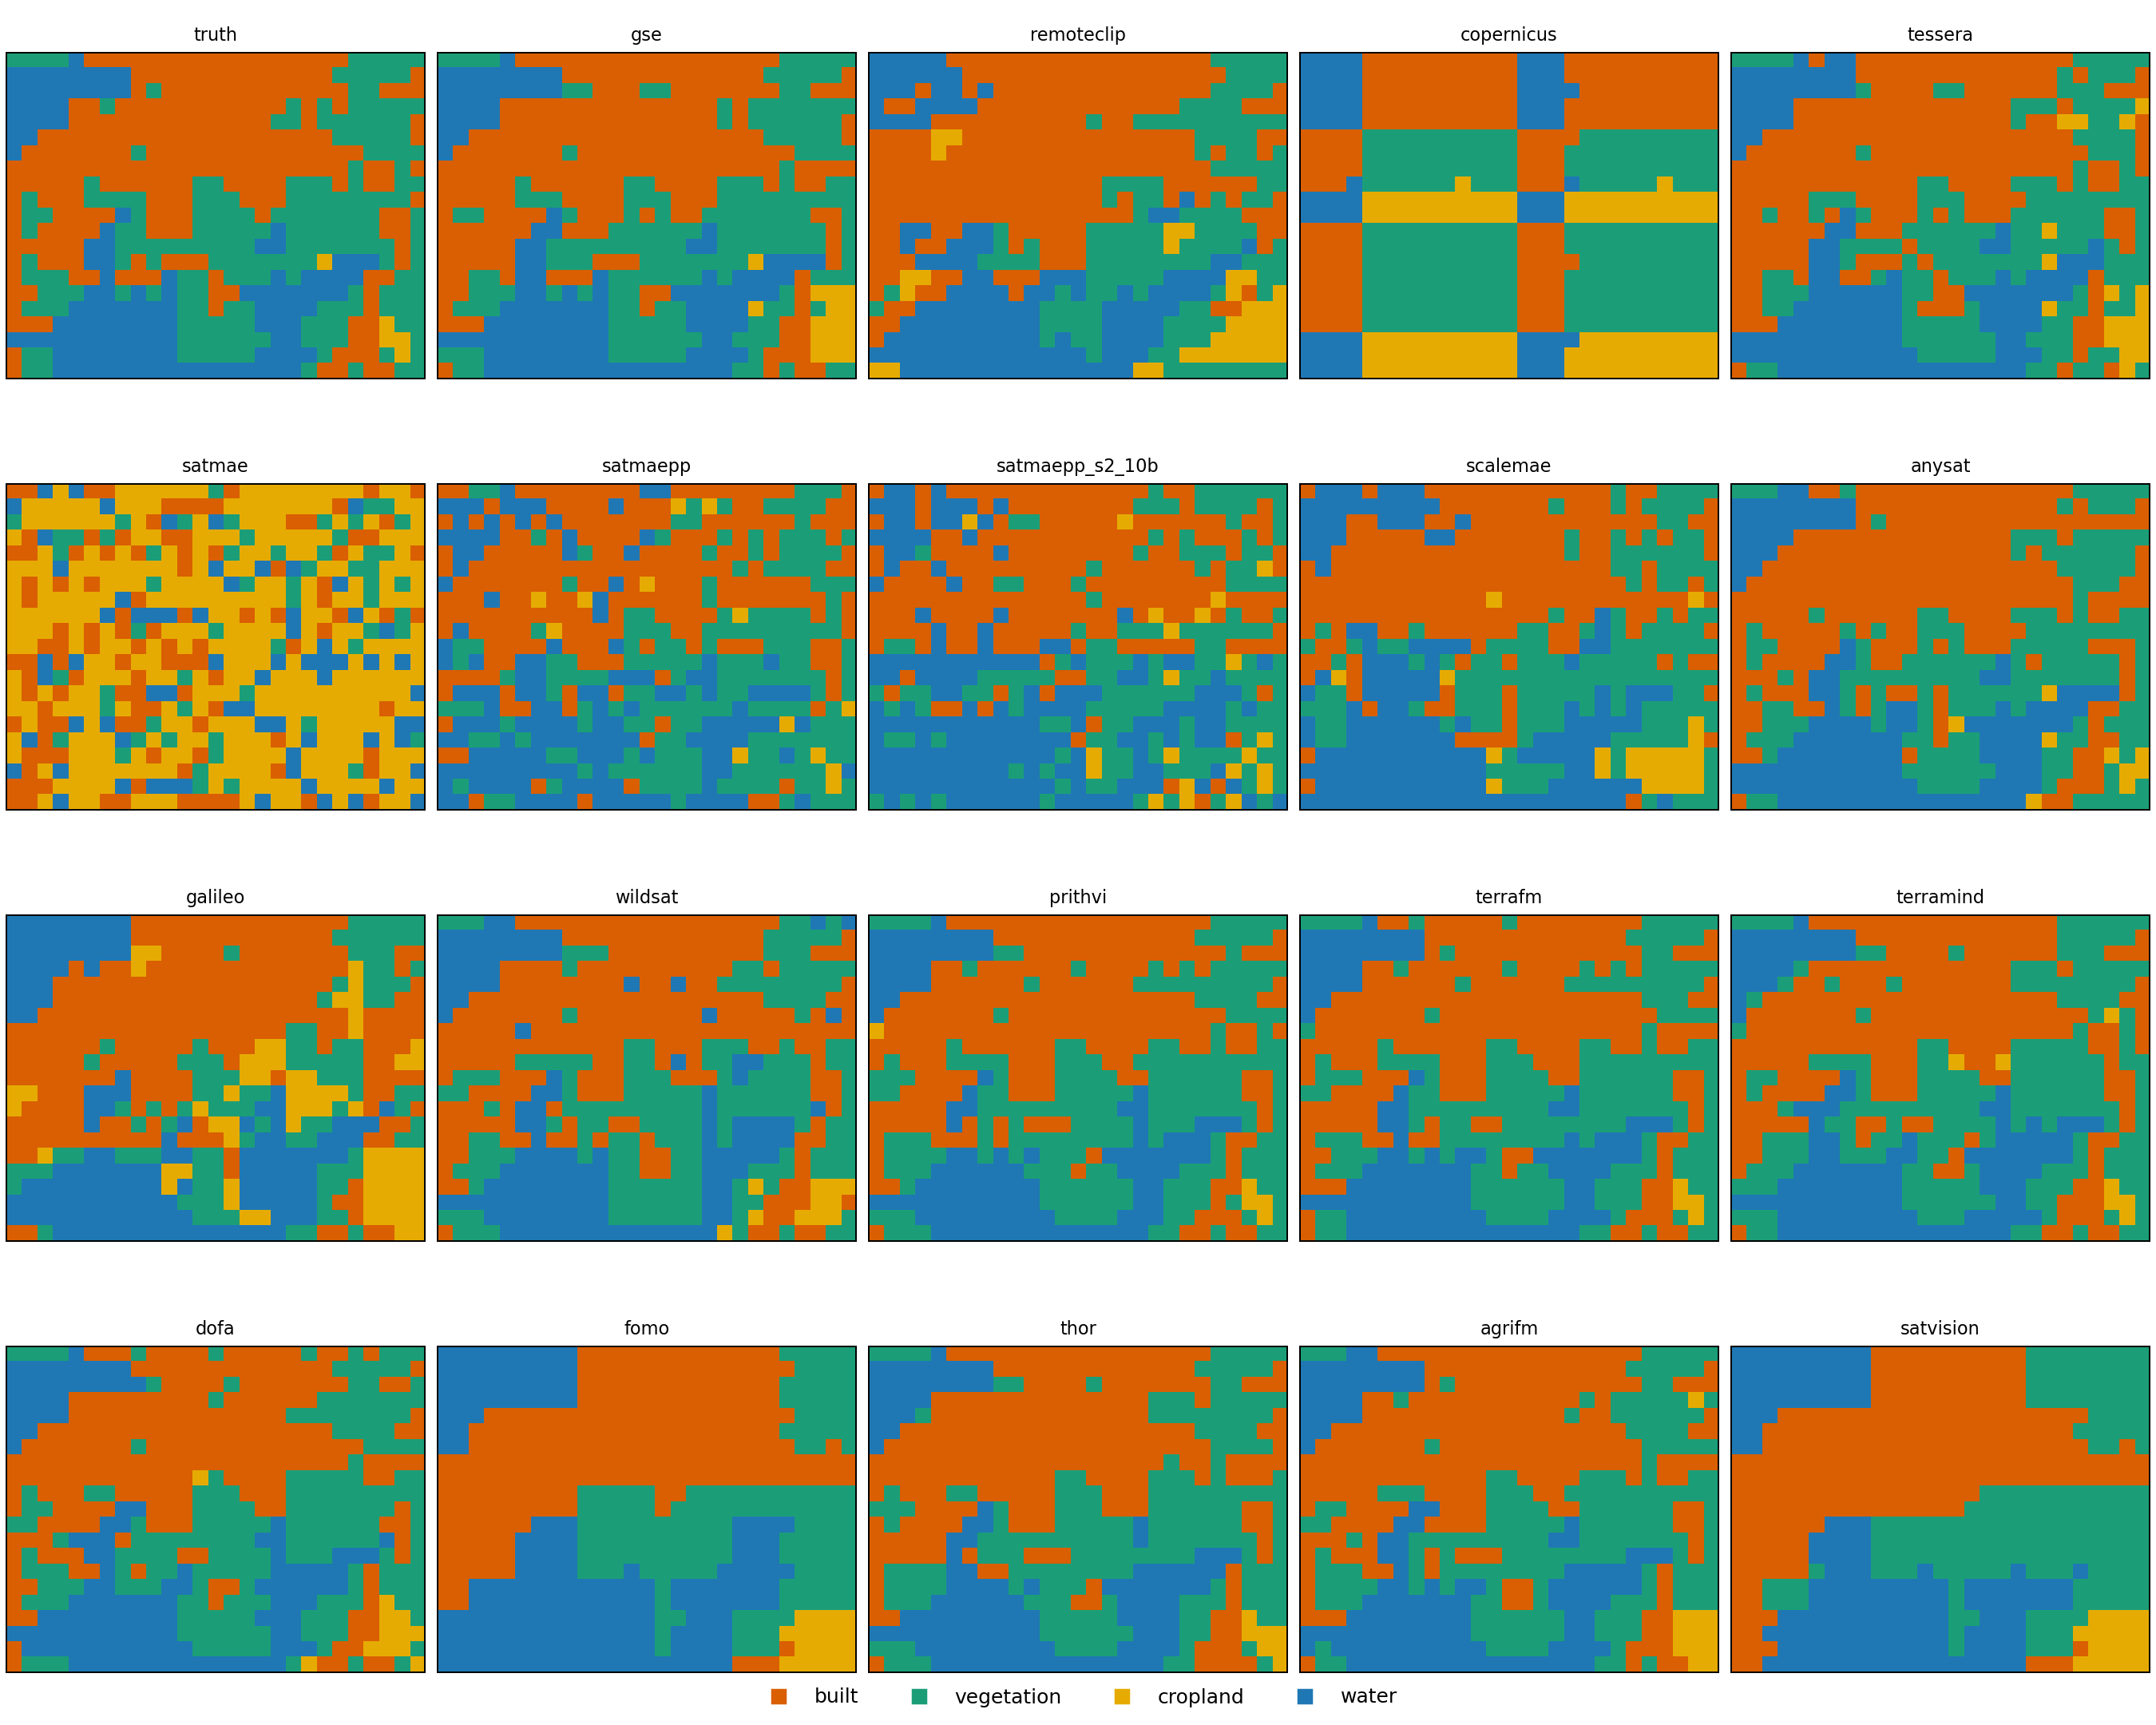
\includegraphics[width=\textwidth]{fig12_wuhan_2x_classification_maps.png}
  \caption{Per-model classification maps for the two-by-two Wuhan benchmark
  window. Each panel uses the same 500\,m tile grid and split-derived probe,
  allowing spatial errors and over-smoothing to be compared across all
  \modelcount{} public models.}
  \label{fig:wuhan-2x-classification-maps}
\end{figure}

The fraction-regression task evaluates a complementary property: whether the embedding preserves smoothly varying land-cover composition rather than only a dominant class label. Using ridge probes over built-up, vegetation, cropland, and water fractions, GSE again ranks first with a mean test Spearman correlation of 0.881 (\figref{fig:wuhan-2x-fraction-spearman}). TESSERA and THOR follow closely at 0.866 and 0.852, while DOFA, TerraMind, AgriFM, Prithvi, AnySat, and TerraFM remain in a competitive middle band. The strongest models are especially consistent for built-up and vegetation fractions, where several models exceed 0.90 Spearman correlation. Cropland and water are harder in this urban-lake corridor, producing wider differences across models and making the mean score a useful summary of robustness across target variables. \figref{fig:wuhan-2x-fraction-scatter} gives the point-level view behind the ranking. In the strongest panels, the cloud of points follows the one-to-one diagonal for built-up and vegetation fractions, indicating that the probe is not only ordering tiles correctly but also recovering approximate sub-tile proportions. The middle-tier models retain the main monotonic trend but show broader vertical spread, especially for cropland and water. The weakest models show compressed predictions or diffuse point clouds, meaning that their embeddings contain less recoverable information about continuous land-cover mixture in this local setting.

\begin{figure}[t]
  \centering
  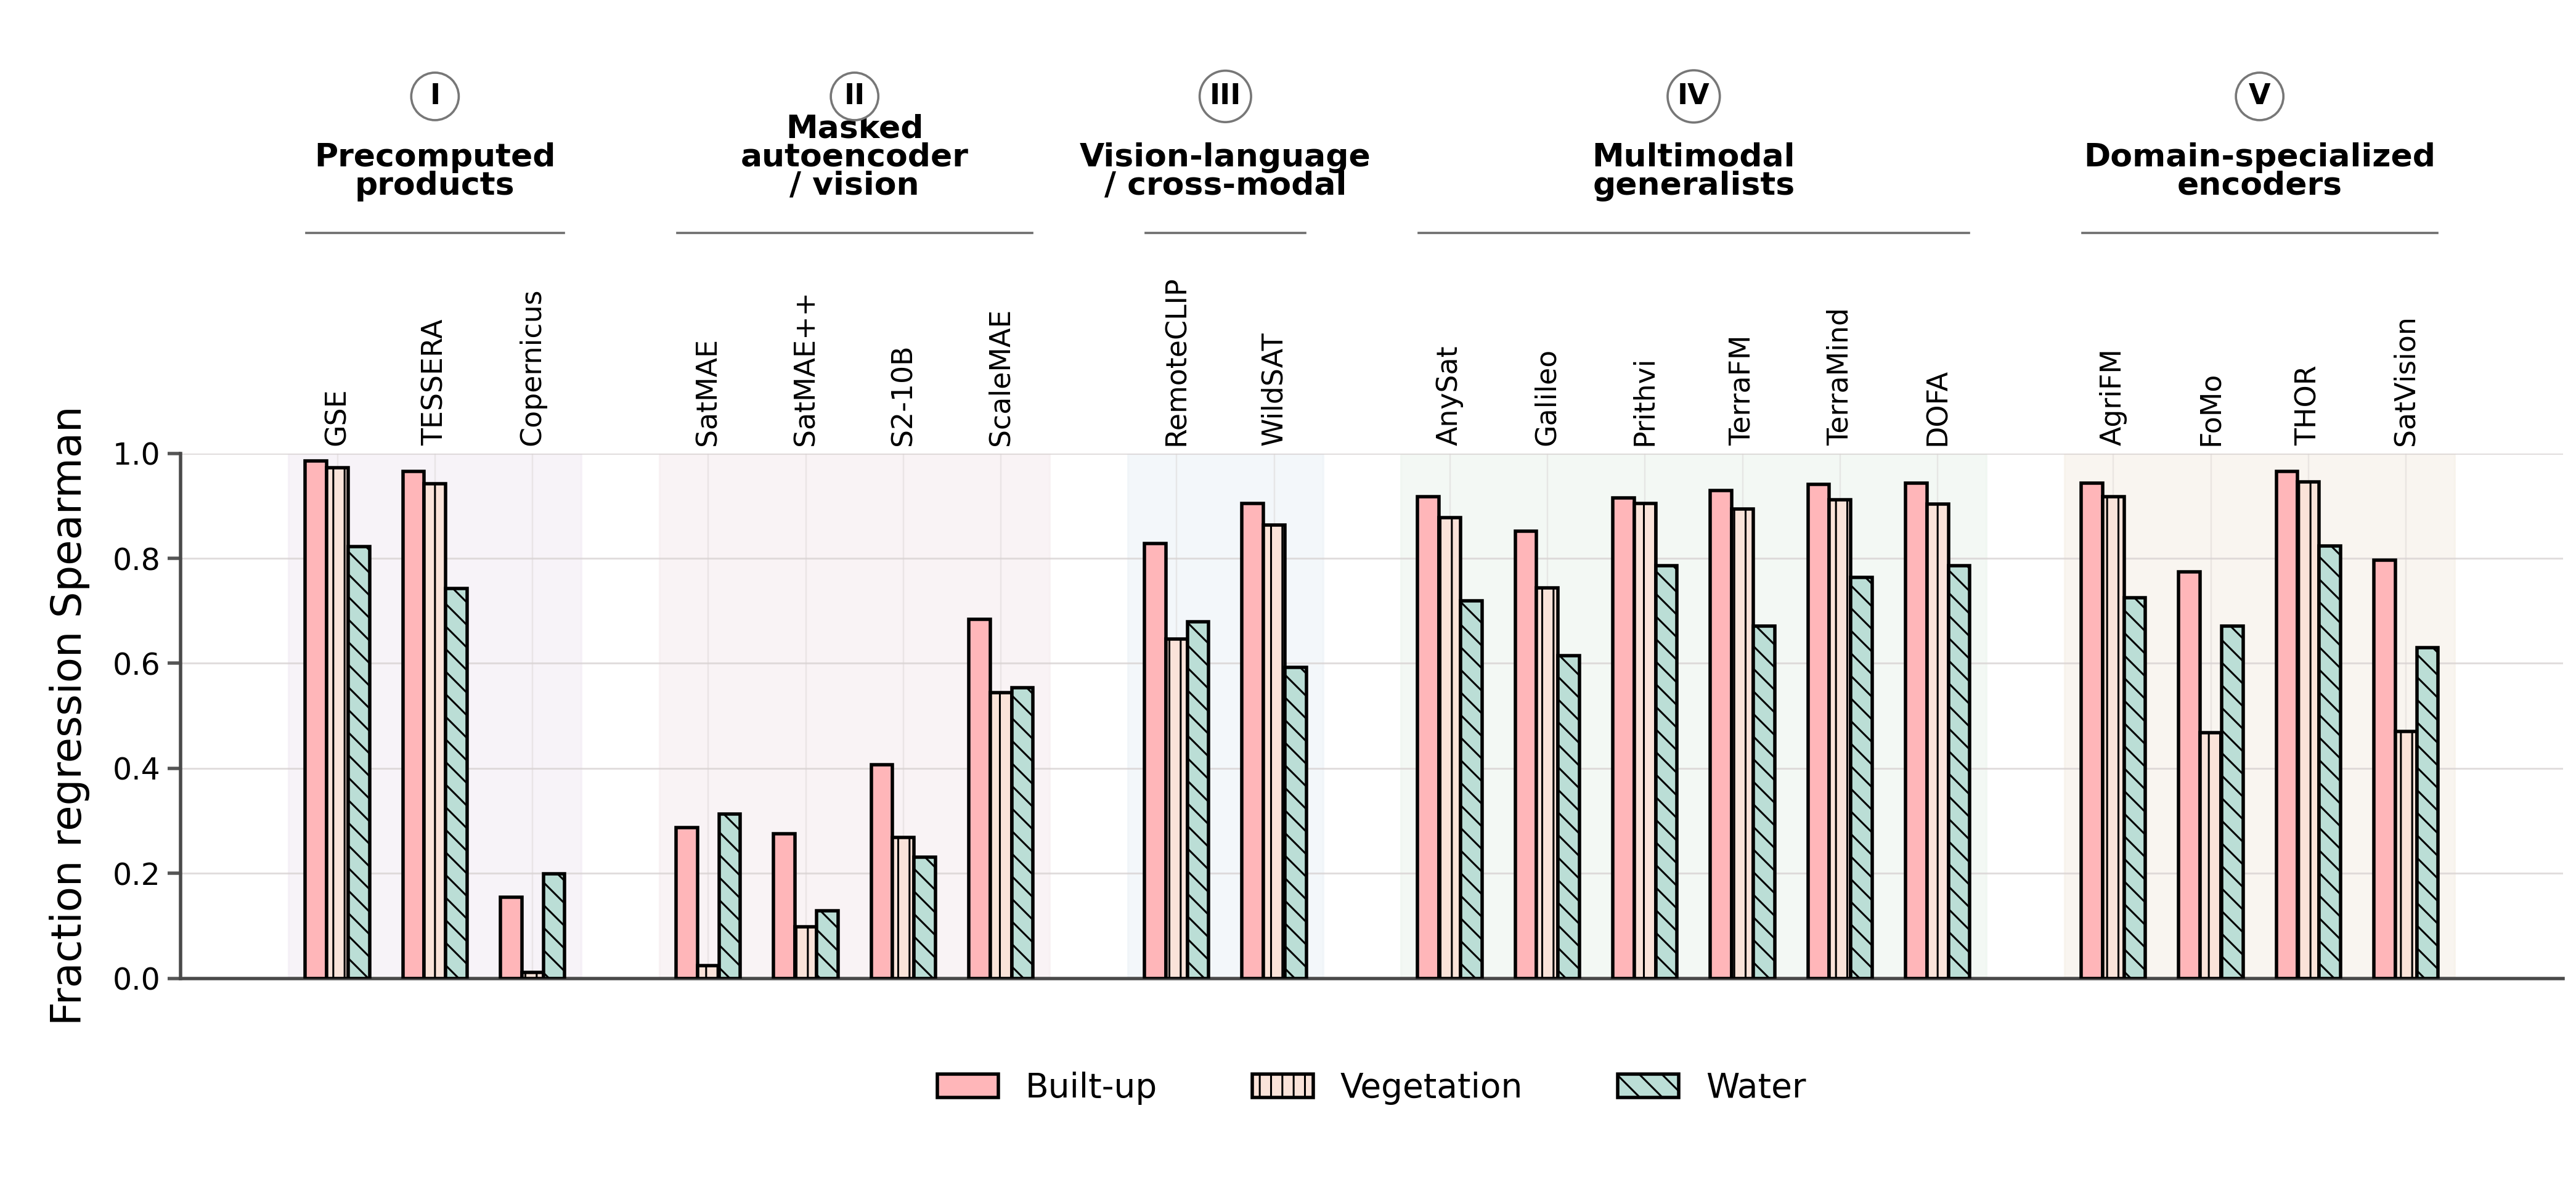
\includegraphics[width=\textwidth]{fig14_wuhan_2x_fraction_spearman.png}
  \caption{Fraction-regression performance on the two-by-two Wuhan benchmark
  window. Bars summarize test Spearman correlation across built-up,
  vegetation, cropland, and water fraction targets using cached public-model
  embeddings and ridge regression probes.}
  \label{fig:wuhan-2x-fraction-spearman}
\end{figure}

\figref{fig:wuhan-2x-fraction-scatter} gives the point-level view behind
the regression ranking. In the strongest panels, the cloud of points follows the
one-to-one diagonal for built-up and vegetation fractions, indicating that the
probe is not only ordering tiles correctly but also recovering approximate
sub-tile proportions. GSE, TESSERA, and THOR show the tightest alignment across
targets, which is consistent with their leading mean Spearman scores. The
middle-tier models retain the main monotonic trend but show broader vertical
spread, especially for cropland and water. The weakest models show compressed
predictions or diffuse point clouds, meaning that their embeddings contain less
recoverable information about continuous land-cover mixture in this local
setting. Read together with \figref{fig:wuhan-2x-fraction-spearman}, the
scatter plot clarifies that high regression performance corresponds to both
rank consistency and visually calibrated fraction estimates, rather than to a
single averaged leaderboard value.

\begin{figure}[t]
  \centering
  \includegraphics[width=\textwidth]{fig13_wuhan_2x_fraction_scatter.png}
  \caption{Predicted versus reference fraction-regression scatter plots for all
  public models on the two-by-two Wuhan benchmark. The panels diagnose whether
  continuous land-cover proportions are preserved in the frozen embeddings
  beyond dominant-class classification.}
  \label{fig:wuhan-2x-fraction-scatter}
\end{figure}

Water extraction isolates a more operational decision. A tile is treated as water when at least half of its area is covered by the JRC-derived binary water mask, yielding 185 positive tiles out of 567 in the two-by-two Wuhan window. Unlike fraction regression, this task asks whether a frozen embedding can support a threshold-like water/non-water decision with a lightweight linear probe. \figref{fig:wuhan-2x-water-metrics} shows that DOFA is the strongest model on this binary extraction task, reaching 0.895 test IoU and 0.944 F1. THOR, TerraMind, TerraFM, TESSERA, GSE, AnySat, Prithvi, and AgriFM form a strong middle-to-high group, all above 0.75 IoU. The map panels in \figref{fig:wuhan-2x-water-maps} provide the spatial counterpart to the leaderboard: high-performing models recover the continuous lake corridor and suppress most built-up or vegetated non-water tiles, while weaker models either over-predict water along mixed boundaries or miss smaller water-adjacent tiles. This task is useful because it sits between coarse classification and dense segmentation. It is operationally meaningful, yet still compatible with pooled tile embeddings for all public models.

\begin{figure}[t]
  \centering
  \includegraphics[width=\textwidth]{fig15_wuhan_2x_water_extraction_metrics.png}
  \caption{Water extraction performance on the two-by-two Wuhan benchmark
  window. Bars report test IoU, F1, and accuracy for frozen public-model
  embeddings with a CUDA-trained linear binary probe over the shared 500\,m
  tile split.}
  \label{fig:wuhan-2x-water-metrics}
\end{figure}

The map panels in \figref{fig:wuhan-2x-water-maps} provide the spatial
counterpart to the water-extraction leaderboard. High-performing models recover
the continuous lake corridor and suppress most built-up or vegetated non-water
tiles, while weaker models either over-predict water along mixed boundaries or
miss smaller water-adjacent tiles. This visual diagnostic is important because
binary IoU alone cannot distinguish a coherent shoreline error from scattered
false positives. Together, the metric and map views show that water extraction
is a useful intermediate task between coarse tile classification and dense
segmentation: it is operationally meaningful, but still compatible with pooled
tile embeddings for all \modelcount{} public models.

\begin{figure}[t]
  \centering
  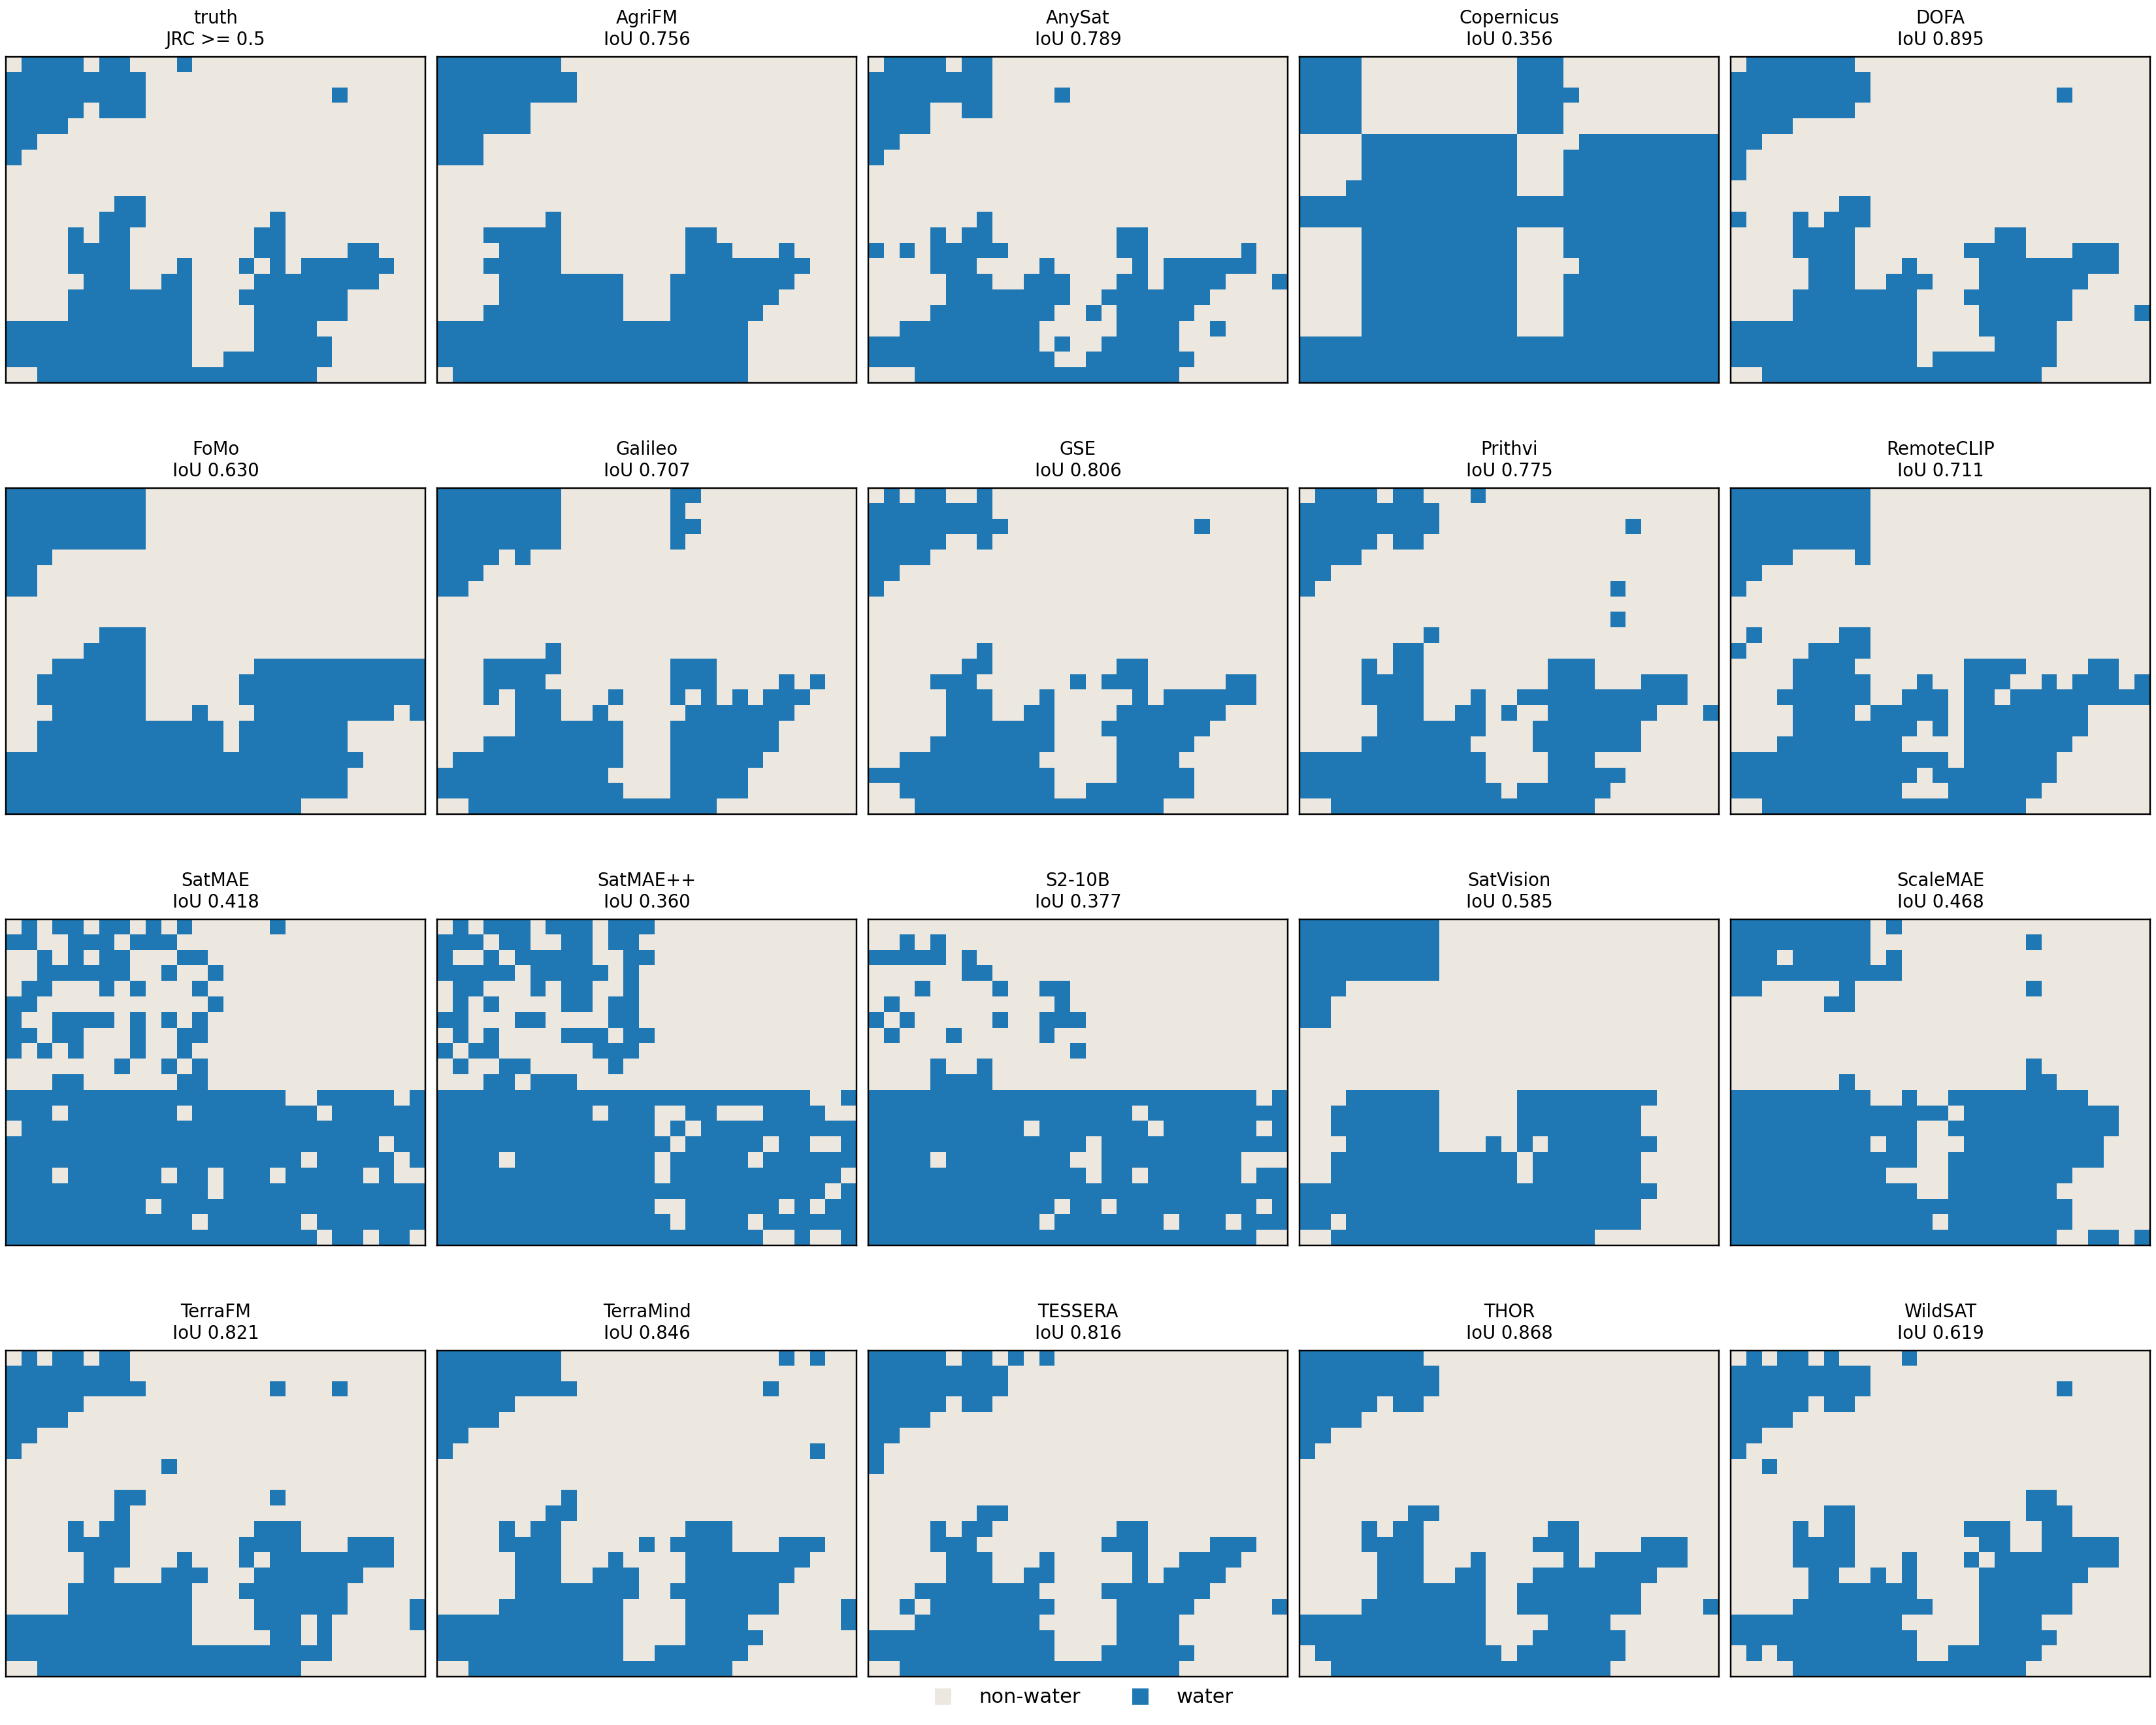
\includegraphics[width=\textwidth]{fig16_wuhan_2x_water_extraction_maps.png}
  \caption{JRC water truth and public-model water-extraction maps for the
  two-by-two Wuhan benchmark window. Each model predicts water/non-water labels
  on the same 500\,m tile grid, making shoreline coherence and false-positive
  patterns directly comparable across all \modelcount{} public models.}
  \label{fig:wuhan-2x-water-maps}
\end{figure}

The final task moves from binary water extraction to dense multi-class segmentation. Here the target is the four-class WorldCover-derived mask used throughout the benchmark: built-up, vegetation, cropland, and water. For each model, class prototypes are estimated from prompted pixels in the dense embedding grid, class-specific thresholds are calibrated on the validation split, and the resulting mask is evaluated on the held-out test split. This is closer to a SAM-style use of embeddings than the preceding probe tasks: the model is not trained end-to-end for segmentation, but its dense representation is queried with class prompts and converted into a mask by thresholding. \figref{fig:wuhan-2x-multiclass-seg-metrics} shows that GSE is the clear leader for this dense multi-class setting, reaching 0.615 test mIoU, 0.700 macro-F1, and 0.833 accuracy. TESSERA ranks second with 0.503 mIoU, followed by AnySat and AgriFM. The class-wise scores reveal an important asymmetry: water is recovered well by the leading models, while cropland remains difficult because it occupies a small and spatially mixed portion of the two-by-two window. \figref{fig:wuhan-2x-multiclass-seg-maps} makes this asymmetry visible. GSE and TESSERA preserve the strongest correspondence to the WorldCover reference, especially for the lake and larger built-up or vegetated zones. AnySat and AgriFM recover the broad water and green structure but lose more detail at class boundaries. Several lower-ranked models collapse toward one or two dominant classes, showing that their dense maps contain less separable class information under this prompt-threshold protocol.

\begin{figure}[t]
  \centering
  \includegraphics[width=\textwidth]{fig17_wuhan_2x_multiclass_segmentation_metrics.png}
  \caption{SAM-like multi-class threshold segmentation on the two-by-two Wuhan
  benchmark window. Bars report test mIoU, macro-F1, and accuracy for
  built-up, vegetation, cropland, and water masks derived from dense public
  embeddings with validation-calibrated class thresholds.}
  \label{fig:wuhan-2x-multiclass-seg-metrics}
\end{figure}

The maps in \figref{fig:wuhan-2x-multiclass-seg-maps} make these
differences visible. GSE and TESSERA preserve the strongest correspondence to
the WorldCover reference, especially for the lake and larger built-up or
vegetated zones. AnySat and AgriFM recover the broad water and green structure
but lose more detail at class boundaries. Several lower-ranked models collapse
toward one or two dominant classes, showing that their dense maps contain less
separable class information under this prompt-threshold protocol. Copernicus is
again a scale-mismatch failure case: its native product grid is too coarse for a
local dense segmentation benchmark of this size.

\begin{figure}[t]
  \centering
  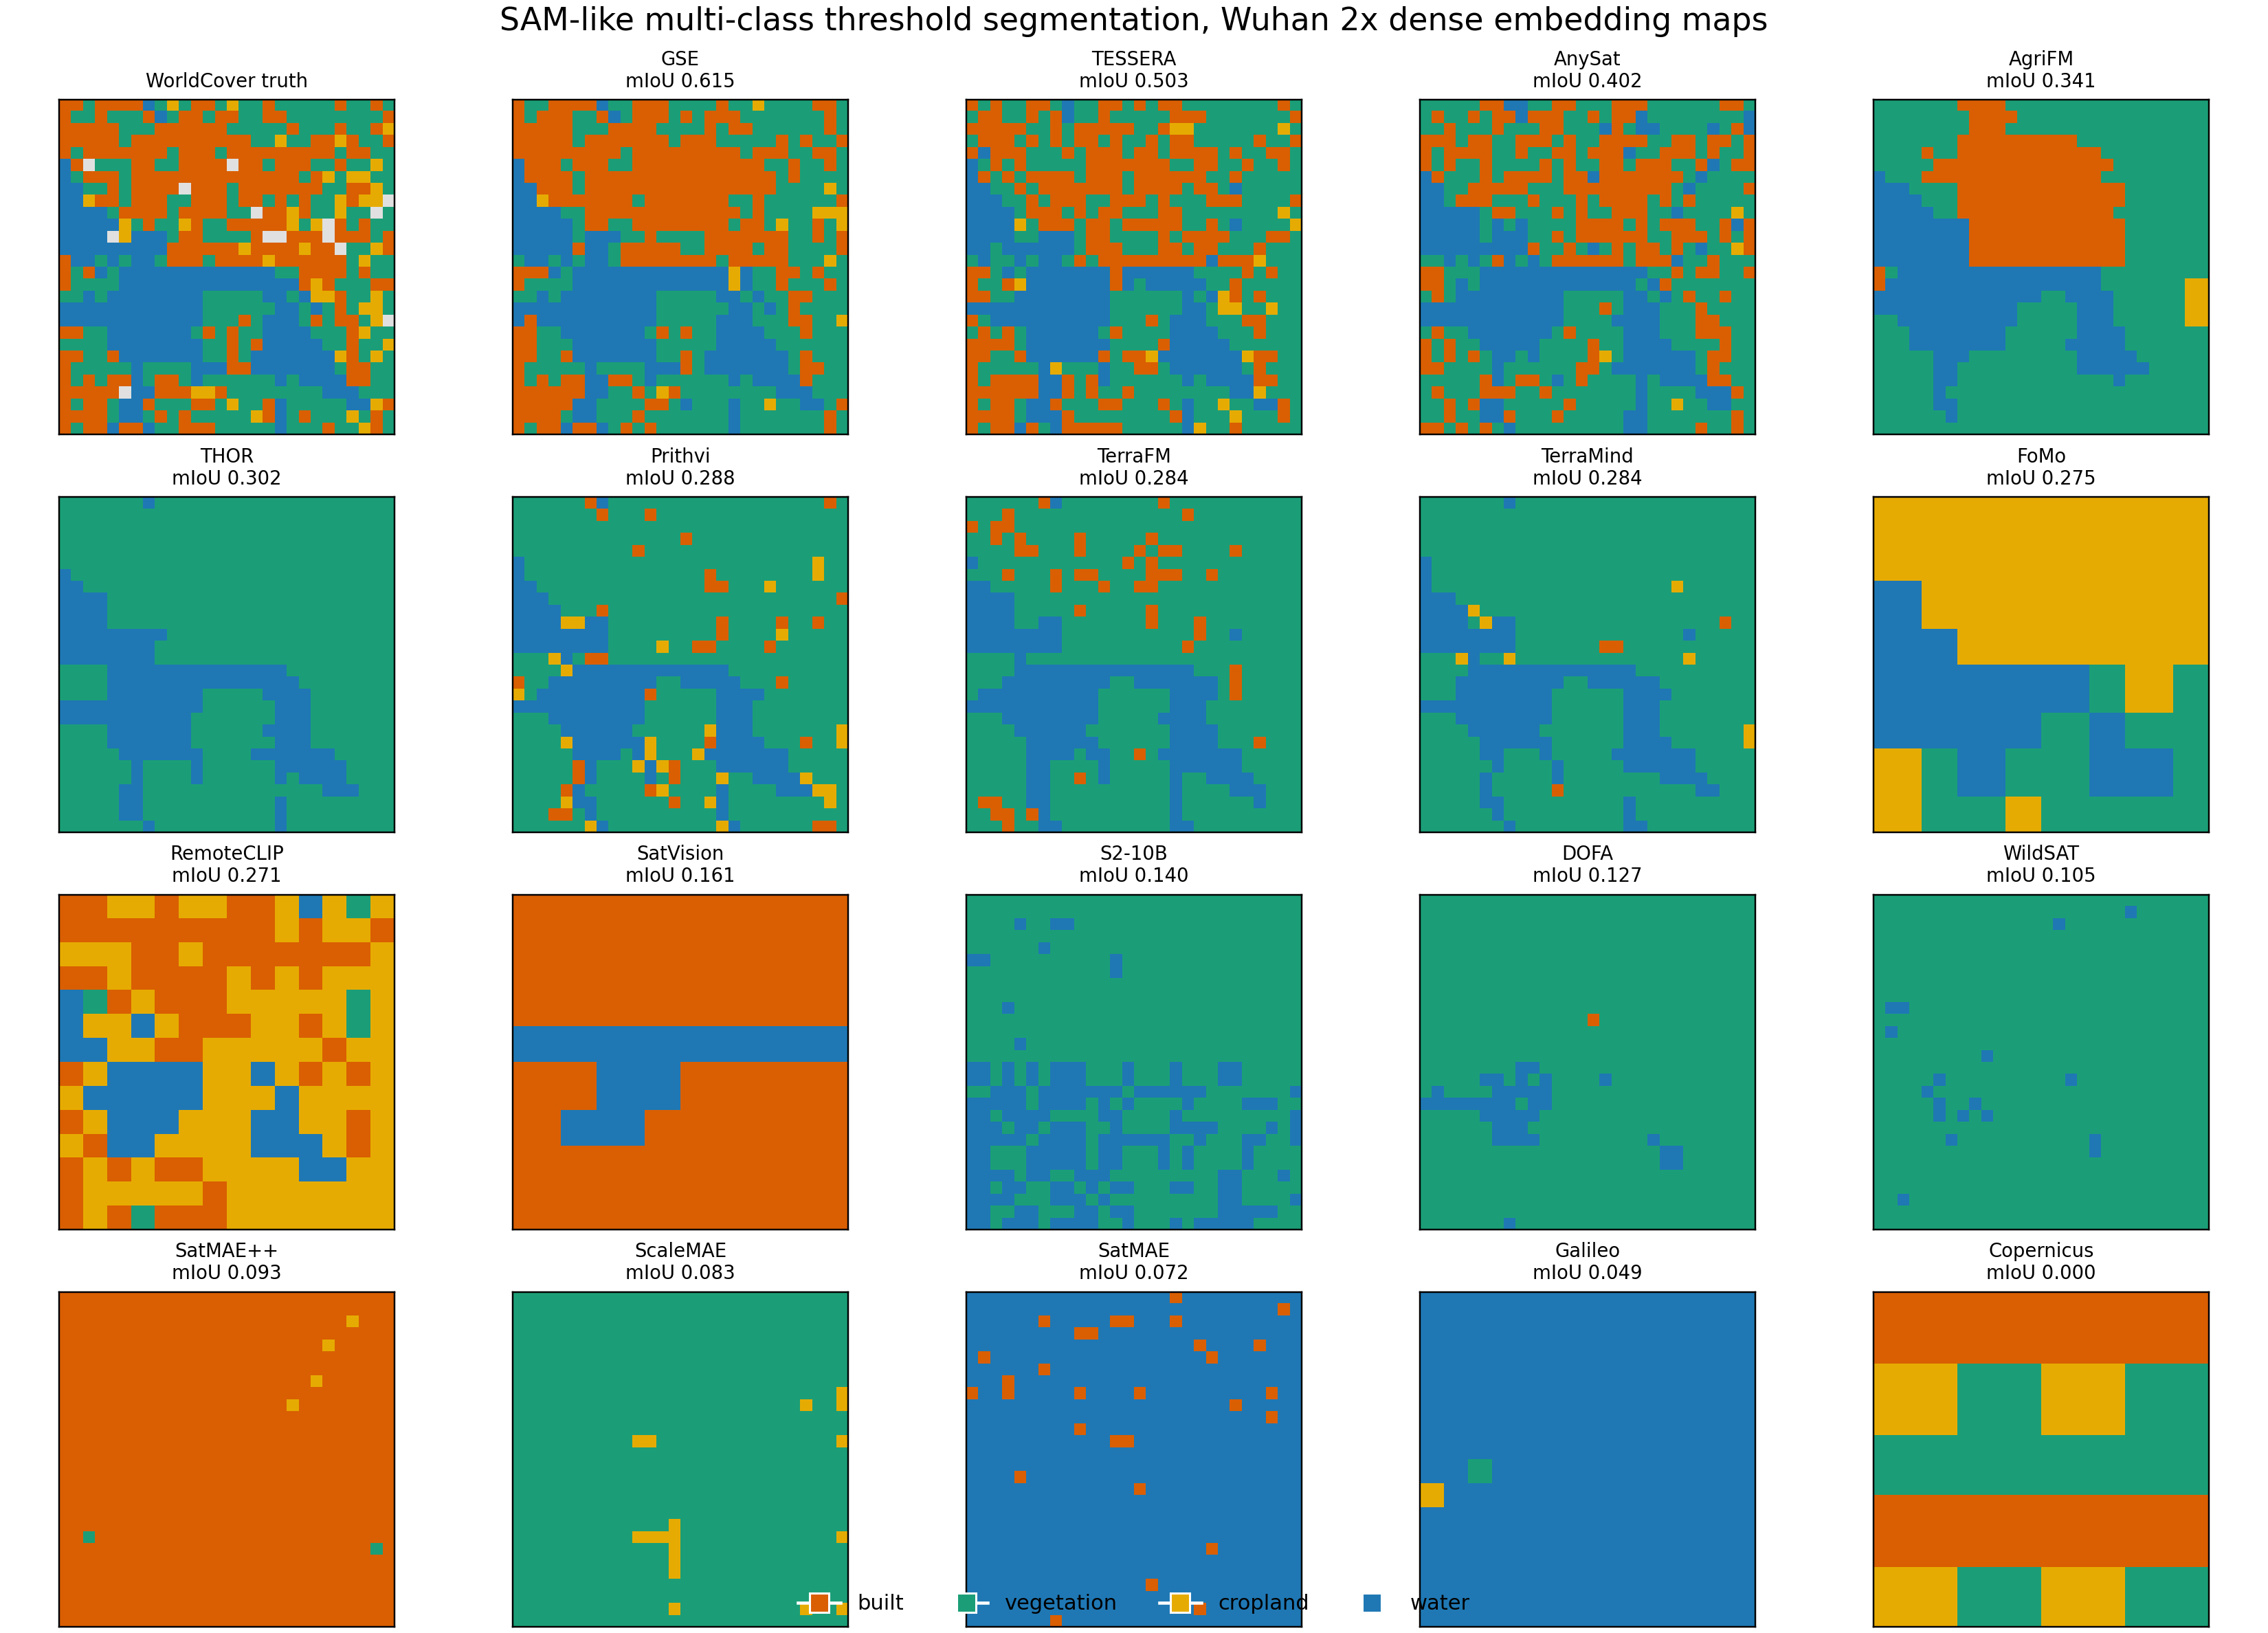
\includegraphics[width=\textwidth]{fig18_wuhan_2x_multiclass_segmentation_maps.png}
  \caption{WorldCover truth and public-model multi-class threshold
  segmentation maps for the two-by-two Wuhan benchmark window. Panels use the
  same four classes---built-up, vegetation, cropland, and water---so class
  collapse, boundary errors, and scale mismatch can be visually compared across
  all \modelcount{} public models.}
  \label{fig:wuhan-2x-multiclass-seg-maps}
\end{figure}

Across the four tasks, three conclusions are more important than the exact ordering of every model. First, productized and multimodal embeddings are highly competitive in this local setting. GSE is the strongest or near-strongest model in classification, fraction regression, and dense segmentation, while TESSERA, THOR, DOFA, TerraMind, AnySat, and AgriFM recur in the upper or middle tiers depending on the task. Second, the benchmark repeatedly exposes scale mismatch. Coarse products or checkpoints whose input assumptions are poorly aligned with a 500\,m local Sentinel-2 window can fail even when they are useful at their native scale. This does not make those models weak in general; it shows that embedding evaluation must respect the spatial unit at which the representation is produced. Third, no single metric captures all useful behavior. Classification highlights dominant semantic separability, regression highlights continuous mixture structure, water extraction highlights operational thresholdability, and dense segmentation highlights local spatial separability. Read together, the Wuhan benchmark supports the main claim of the review: satellite embeddings should be compared as reusable geospatial representations, not only as model names or pretraining recipes.

\clearpage

\section{Open Challenges and Future Directions}

The review and Wuhan benchmark point to several challenges that are now becoming central for satellite embeddings. The first is temporal ambiguity. Many current systems use the same word, embedding, for annual products, short seasonal composites, single-date observations, and multi-step time series. These objects can all be useful, but they do not preserve the same temporal information. A representation that averages a year of observations may be stable for land-cover mapping but poorly suited to flood response or phenology-sensitive agriculture; a temporal encoder may preserve seasonal dynamics but require inputs that are difficult to obtain in cloudy or data-sparse regions; a precomputed product may be easy to sample but locked to the upstream production calendar. Future papers should therefore report not only the sensor and spatial resolution of an embedding, but also its temporal support, compositing rule, update frequency, and intended interpretation. This would make model selection more transparent and would prevent annual products, scene encoders, and temporal sequence models from being compared as if they were the same representation.

The second challenge is scale mismatch. Remote sensing reviews have long emphasized that spatial, spectral, and temporal resolution determine what can be observed, but foundation-model discussions sometimes hide this fact behind architecture names. The Wuhan benchmark makes the issue concrete: embeddings produced at 10\,m, 30\,m, 500\,m, 1\,km, or 0.25$^\circ$ are not interchangeable, and resampling cannot create local information that was never present in the native representation. This is especially important for precomputed products because their convenience can encourage users to sample them outside the scale at which they are meaningful. A stronger evaluation culture would report native support, resampling choices, and target grid size together with accuracy. It would also include visual diagnostics, because map coherence often reveals scale failure before a single aggregate metric does.

The third challenge is the comparison between products and checkpoints. Precomputed embedding fields optimize access, coverage, and repeatability; on-the-fly encoders optimize flexibility, temporal control, and adaptation to new inputs. Both are legitimate satellite embedding regimes, but they should not be evaluated only by the same predictive score. Product models should be credited for low inference burden, stable large-area sampling, and reproducible feature layers. Checkpoint models should be credited for sensor-specific control, temporal customization, dense readout options, and the ability to adapt to new data streams. Future benchmarks should therefore pair quality metrics with deployment metrics such as extraction latency, GPU memory, missing-data behavior, storage footprint, and product availability. This is not an engineering afterthought. For Earth observation, these constraints often decide whether a representation can be used at continental scale or in repeated monitoring.

The fourth challenge is application realism. Standard remote sensing datasets remain valuable, but satellite embeddings are increasingly used in settings that do not look like benchmark leaderboards: sparse labels, mixed pixels, shifting seasons, changing sensors, region transfer, and continuous environmental quantities. The Wuhan benchmark is only a first step, yet it shows why related task families are useful. Classification, regression, water extraction, and segmentation expose different failure modes over the same region. Future work should extend this logic to larger and more diverse ROIs, cross-year splits, few-label protocols, and physically meaningful regression targets such as canopy height, biomass, crop condition, surface water dynamics, and urban intensity. The field also needs clearer reporting of negative results. A model that fails because of scale mismatch, unavailable inputs, or temporal misalignment teaches a different lesson from a model that fails because its representation is weak.

Finally, satellite embeddings need more standardized reporting. A useful model card for this area should include the pretraining data regime, sensor assumptions, native spatial and temporal support, output forms, embedding dimensionality, dense-readout availability, licensing or product access, and recommended downstream usage. Recent systems such as Prithvi-EO-2.0 and FlexiMo show that the field is continuing to expand toward more flexible multitemporal and multimodal representations \citep{prithvieo2_tgrs,fleximo_tgrs}. As that expansion continues, the review problem will become less about whether a model is a foundation model and more about whether its embedding is the right geospatial object for a given task. The next generation of surveys should therefore combine taxonomy, evidence, and reporting standards rather than treating model inventories as sufficient.

\section{Conclusion}

Satellite embeddings are becoming a practical abstraction layer for Earth observation. They connect large archives, foundation-model training, precomputed products, and lightweight downstream analysis, but the literature still tends to describe them indirectly through model families or benchmark datasets. This review argues for a more direct framing: the reusable representation itself should be the unit of organization. From that perspective, precomputed products, masked autoencoders, vision-language encoders, multimodal generalists, and domain-specialized models can be compared as different ways of producing transferable geospatial features under different sensing assumptions.

The main contribution of the review is therefore twofold. First, it provides an embedding-centered taxonomy and model dossier for \modelcount{} representative public models, making sensor support, temporal semantics, output form, dimensionality, and deployment mode visible alongside architecture and pretraining objective. Second, it links that taxonomy to a compact Wuhan benchmark that evaluates frozen embeddings under shared geographic, label, and probe conditions. The results show that model choice depends on the target property being tested: semantic separability, continuous land-cover mixture, water thresholdability, and dense spatial separability emphasize different strengths and weaknesses. They also show that scale mismatch is not a minor implementation detail, but a central factor in whether an embedding is meaningful for local mapping.

The broader lesson is that satellite embeddings should be selected and evaluated as geospatial representations, not only as checkpoints. A useful review must therefore connect literature synthesis with data regimes, application requirements, operational constraints, and empirical diagnostics. The current paper is a step in that direction: it keeps the broad survey structure of recent remote sensing reviews, but adds an embedding-specific benchmark lens that makes representation behavior visible in one controlled ROI. Future extensions should scale this evidence across regions, years, and physically grounded regression targets while preserving the same principle: compare embeddings in the form practitioners actually use them.


\bibliographystyle{plainnat}
\bibliography{references}

\end{document}